%\documentclass{beamer}
%\usepackage{amsmath}
%\usepackage{amsfonts}
%\usepackage{amsthm}
%\usepackage{amssymb}
%\usepackage{tikz}
%\usetikzlibrary{trees}

%===== main document class =====
%\ifdefined\slideModeHandout
\documentclass%
[%
  handout,          % avoid unnecessary overlays
  aspectratio=169,  % aspect ratio fo 16:9 
  t,                % place content at top of frames
  10pt,             % use 10pt as standard font size (default size is 11pt)
  compress,         % compress things like navigation bars...
]{beamer}
%\else
%\documentclass%
%[%
%  aspectratio=169,  % aspect ratio fo 16:9 
%  t,                % place content at top of frames
%  10pt,             % use 10pt as standard font size (default size is 11pt)
%  compress,         % compress things like navigation bars...
%]{beamer}
%\fi

\mode<presentation>
%===============tabto==============
% tabto.sty
%
% version 1.4  (Dec 2018)
%
% Tabbing to fixed positions in a paragraph.
%
% Copyright 2006,2009,2012,2013,2018 by 
% Donald Arseneau,   Vancouver, Canada (asnd@triumf.ca)
% Permission to use, distribute and modify this software is granted
% under the conditions of the LaTeX Project Public License, either 
% version 1.3 or (at your option) any later version.  The license is
% found at http://www.latex-project.org/lppl.txt, and is part of all 
% recent distributions of LaTeX.
%
% This work has the LPPL maintenance status `maintained' (by author).
%
% Two new text positioning commands are defined: \tabto and \tab.
% 
% \tabto{<length>}
% Tab to a position relative to the left margin in a paragraph (any
% indentation due to a list or \leftskip is part of the `margin' in
% this context). If the text on the line already goes past the desired
% position, the tab starts a new line and moves to the requested
% horizontal position.
%
% \tabto*{<length>}
% Similar to \tabto, except it will perform backspacing, and over-
% print previous text on the line whenever that text is already
% longer than the specified length (i.e., no linebreak is produced).
% Line-breaks are suppressed immediately after \tabto or \tabto*.
%
% The length register "\CurrentLineWidth" will report the width
% of the existing text on the line, and it may be used in the
% <length> argument (using calc.sty, for example). Also, there
% is "\TabPrevPos" which gives the "\CurrentLineWidth" from the
% previous tab command (the position where the tab command occurred,
% not where it went to), and can be used to return to that position
% if no line breaks have occurred in between, or directly below it,
% if there were line breaks.
%
% \tab
% Tab to the next tab-stop chosen from a list of tab positions, in
% the traditional style of typewriters.  A \tab will always move
% to the next tab stop (or the next line), even if it is already
% exactly at a tab stop. Thus, "\tab" at the beginning of a line,
% or "\tab\tab" elsewhere skips a position. A linebreak is permitted 
% immediately following a \tab, in case the ensuing text does not 
% fit well in the remaining space.
%
% If you do not want to skip positions, use "\tabto{\NextTabStop}"
% instead of "\tab".  This is particularly useful when you want to
% use \tab in some other command, but do not want to skip a column
% for the first item.
%
% The tab-stop positions are declared using either \TabPositions
% or \NumTabs:
%
% \TabPositions{<length>, <length>,...<length>}
% Declares the tab stops as a comma-separated list of positions 
% relative to the left margin. A tab-stop at 0pt is implicit, and 
% need not be listed.
%
% \NumTabs{<number>}
% Declares a list of <number> equally-spaced tabs, starting at the
% left margin and spanning \linewidth.  For example \NumTabs{2} 
% declares tab-stops at 0pt and 0.5\linewidth, the same as
% \TabPositions{0pt, 0.5\linewidth} or \TabPositions{0.5\linewidth}
%
% After these declarations, the list of tab positions is saved in
% \TabStopList, and the next tab position, relative to the current 
% position, is given by \NextTabStop.  You do not normally need
% to access them, but they are available.
%
% Problems:
%
% Tall objects after a tab stop may overlap the line above, rather
% than forcing a greater separation between lines.

%\ProvidesPackage{tabto}[2018/12/28 \space v 1.4 \space 
%  Another tabbing mechanism]\relax

%%%%%%%%%Code Begin

%\newdimen\CurrentLineWidth
%\newdimen\TabPrevPos
%
%\newcommand\tabto[1]{%
% \leavevmode
% \begingroup
% \def\@tempa{*}\def\@tempb{#1}%
% \ifx\@tempa\@tempb % \tab* 
%   \endgroup
%   \TTo@overlaptrue % ... set a flag and re-issue \tabto to get argument
%   \expandafter\tabto
% \else
%   \ifinner % in a \hbox, so ignore
%   \else % unrestricted horizontal mode
%     \null% \predisplaysize will tell the position of this box (must be box)
%     \parfillskip\fill
%     \everydisplay{}\everymath{}%
%     \predisplaypenalty\@M \postdisplaypenalty\@M
%     $$% math display so we can test \predisplaysize
%      \lineskiplimit=-999pt % so we get pure \baselineskip
%      \abovedisplayskip=-\baselineskip \abovedisplayshortskip=-\baselineskip
%      \belowdisplayskip\z@skip \belowdisplayshortskip\z@skip
%      \halign{##\cr\noalign{%
%        % get the width of the line above
%        \ifdim\predisplaysize=\maxdimen %\message{Mixed R and L, so say the line is full. }%
%           \CurrentLineWidth\linewidth
%        \else
%           \ifdim\predisplaysize=-\maxdimen 
%             % \message{Not in a paragraph, so call the line empty. }%
%             \CurrentLineWidth\z@
%           \else
%             \ifnum\TTo@Direction<\z@
%               \CurrentLineWidth\linewidth \advance\CurrentLineWidth\predisplaysize
%             \else
%               \CurrentLineWidth\predisplaysize 
%             \fi
%             % Correct the 2em offset
%             \advance\CurrentLineWidth -2em
%             \advance\CurrentLineWidth -\displayindent
%             \advance\CurrentLineWidth -\leftskip
%        \fi\fi
%        \ifdim\CurrentLineWidth<\z@ \CurrentLineWidth\z@\fi
%        % Enshrine the tab-to position; #1 might reference \CurrentLineWidth
%        \setlength\@tempdimb{#1}% allow calc.sty
%        %\message{*** Tab to \the\@tempdimb, previous width is \the\CurrentLineWidth. ***}%
%        % Save width for possible return use
%        \global\TabPrevPos\CurrentLineWidth
%        % Build the action to perform
%        \protected@xdef\TTo@action{%
%           \vrule\@width\z@\@depth\the\prevdepth
%           \ifdim\CurrentLineWidth>\@tempdimb
%              \ifTTo@overlap\else
%                 \protect\newline \protect\null
%           \fi\fi
%           \protect\nobreak
%           \protect\hskip\the\@tempdimb\relax
%        }%
%        %\message{\string\TTo@action: \meaning \TTo@action. }%
%        % get back to the baseline, regardless of its depth.
%        \vskip-\prevdepth
%        \prevdepth-99\p@
%        \vskip\prevdepth
%      }}%
%      $$
%     % Don't count the display as lines in the paragraph
%     \count@\prevgraf \advance\count@-4 \prevgraf\count@
%     \TTo@action
%     %%   \penalty\@m % to allow a penalized line break
%   \fi
%   \endgroup
%   \TTo@overlapfalse
%   \ignorespaces
% \fi
%}
%
%% \tab -- to the next position
%% \hskip so \tab\tab moves two positions
%% Allow a (penalized but flexible) line-break right after the tab.
%%
%\newcommand\tab{\leavevmode\hskip2sp\tabto{\NextTabStop}%
%  \nobreak\hskip\z@\@plus 30\p@\penalty4000\hskip\z@\@plus-30\p@\relax}
%
%
%% Expandable macro to select the next tab position from the list
%
%\newcommand\NextTabStop{%
%  \expandafter \TTo@nexttabstop \TabStopList,\maxdimen,>%
%}
%
%\def\TTo@nexttabstop #1,{%
%    \ifdim#1<\CurrentLineWidth
%      \expandafter\TTo@nexttabstop
%    \else
%      \ifdim#1<0.9999\linewidth#1\else\z@\fi
%      \expandafter\strip@prefix
%    \fi
%}
%\def\TTo@foundtabstop#1>{}
%
%\newcommand\TabPositions[1]{\def\TabStopList{\z@,#1}}
%
%\newcommand\NumTabs[1]{%
%   \def\TabStopList{}%
%   \@tempdimb\linewidth 
%   \divide\@tempdimb by#1\relax
%   \advance\@tempdimb 1sp % counteract rounding-down by \divide
%   \CurrentLineWidth\z@
%   \@whiledim\CurrentLineWidth<\linewidth\do {%
%     \edef\TabStopList{\TabStopList\the\CurrentLineWidth,}%
%     \advance\CurrentLineWidth\@tempdimb
%   }%
%   \edef\TabStopList{\TabStopList\linewidth}%
%}
%
% %default setting of tab positions:
%\TabPositions{\parindent,.5\linewidth}
%
%%\newif\ifTTo@overlap \TTo@overlapfalse
%
%%\@ifundefined{predisplaydirection}{
%% \let\TTo@Direction\predisplaysize
%% \let\predisplaydirection\@undefined
%%}{
%% \let\TTo@Direction\predisplaydirection
%%}
%
%

% ===== include packages =====
\usepackage{lmodern}
\usepackage[utf8]{inputenc}      % Unicode UTF-8 encoding support
\usepackage[T2A,T1]{fontenc}         % T1 font encoding
\usepackage{etoolbox}            % Programming tools (used for \insertpartstartframe, \insertpartendframe)
\usepackage{ifthen}              % Simple conditional statements
\usepackage{amsmath}             % AMS math package
\usepackage{amssymb}             % Extended collection of math symbols
\usepackage{mathtools}           % More math stuff
\usepackage{nicefrac}            % Nice fractions
\usepackage{xcolor}              % Driver independent colors
\usepackage{colortbl}            % rowcolor for tables
\usepackage{array}               % tables and arrays with extended features (e.g., overlays)
\usepackage{makecell}            % Simple formatting of single table cells
\usepackage{multirow}            % Multi-rows in tabular environments
\usepackage{booktabs}            % More flexible lines for tabular environments
\usepackage{tabto}               % Easy way of specifying tabulators
\usepackage{adjustbox}           % Macros for adjusting boxed content (used in defining \fitbox)
\usepackage{relsize}             % Relative font sizes (\larger=\relsize{1}, \smaller=\relsize{-1})
\usepackage{graphicx}            % Inserting pictures
\usepackage{hyperref}            % Cross referencing
%\usepackage{media9}              % Include media objects
%\usepackage{animate}             % Animations
\usepackage{tikz}                % TikZ library for drawing
\usepackage{pgfplots}            % Plots
\usepackage{import}              % including stuff with relative paths
%\usepackage{listings}            % source code inclusion

%===== TikZ libraries =====
\usetikzlibrary{shapes}          % Additional shapes: Ellipse
\usetikzlibrary{shapes.symbols}  % Additional shapes: Symbols (e.g., "cloud")
\usetikzlibrary{shapes.arrows}   % Additional shapes: Arrows (e.g., "single arrow")
\usetikzlibrary{arrows}          % Arrow tips
\usetikzlibrary{arrows.meta}     % Adjustable arrow heads
\usetikzlibrary{positioning}     % Relative positioning of nodes

%===== pgfsetting =====
\pgfplotsset{compat=newest}      % Use newest version of pgf
\usepgfplotslibrary{fillbetween} % filling between curves

%===== nice tables =====
\setlength{\heavyrulewidth}{0.08em}
\setlength{\lightrulewidth}{0.08em}
\setlength{\cmidrulewidth}{0.04em}
\setlength{\aboverulesep}{0.4ex}
\setlength{\belowrulesep}{0.6ex}
\newcommand{\cmidbeg}{\addlinespace[0.40ex]}
\newcommand{\cmidend}{\addlinespace[0.10ex]}

\usepackage{caption}
\usepackage{subcaption}


%%%%%%%%%%%%%%%%%%%%%%%%%%%%%%%%%%%%%%%%%%%%%%%%%%%%%%%%%%%%
%%%%%%
%%%%%%     M A I N   D O C U M E N T   S W I T C H E S     
%%%%%%
%%%%%%%%%%%%%%%%%%%%%%%%%%%%%%%%%%%%%%%%%%%%%%%%%%%%%%%%%%%%

% define command for directly using switches
\newcommand{\usetoggle}[1]{\iftoggle{#1}{true}{false}}

% define switches
\newtoggle{useNavSymbols}               % display of navigation symbols
\newtoggle{useShadows}                  % use blocks with shadows
\newtoggle{useColorBlocks}              % use colored blocks
\newtoggle{useColorBlockTitles}         % use colored block titles
\newtoggle{useInverseBlockTitles}       % use colored block title background with white text
\newtoggle{altColors}                   % use alternative color theme
\newtoggle{addExercises}                % whether exercises are used
\newtoggle{specialHeiko}                % special stuff for Heiko
\newtoggle{specialThomas}               % special stuff for Thomas

\def\slideStyleThomas{..}


\ifdefined\slideStyleThomas

  %>>>>>>>>>> parameters for Thomas >>>>>>>>>>
  \title%
      [Image and Video Coding]%
      {Image and Video Coding I:\\[0.5ex] Fundamentals}
  \author%
      [T. Wiegand, J. Pfaff, J. Rasch]%
      {Thomas Wiegand, Jonathan Pfaff, Jennifer Rasch}
  \institute%
      [TU Berlin, Fraunhofer HHI]%
      {Technische Universität Berlin, Fraunhofer Heinrich Hertz Institute, Berlin}

  \newcommand{\slideOrganization}{}

  \settoggle{useNavSymbols}        {false}
  \settoggle{useShadows}           {true}
  \settoggle{useColorBlocks}       {true}
  \settoggle{useColorBlockTitles}  {true}
  \settoggle{useInverseBlockTitles}{true}
  \settoggle{altColors}            {false}
  \settoggle{addExercises}         {false}

  \settoggle{specialHeiko}         {false}
  \settoggle{specialThomas}        {true}
  %<<<<<<<<<< parameters for Thomas <<<<<<<<<<

\else

  %>>>>>>>>>> parameters for Heiko >>>>>>>>>>
  \title%
      {Data Compression}
  \author%
      [Heiko Schwarz]%
      {Heiko Schwarz}
  \institute%
      [Freie Universität Berlin]%
      {Freie Universität Berlin\\%
      Fachbereich Mathematik und Informatik}

\ifdefined\slideModeHandout
  \settoggle{useNavSymbols}        {false}
\else
  \settoggle{useNavSymbols}        {false}
\fi
  \settoggle{useShadows}           {true}
  \settoggle{useColorBlocks}       {true}
  \settoggle{useColorBlockTitles}  {true}
  \settoggle{useInverseBlockTitles}{true}
  \settoggle{altColors}            {false}
  \settoggle{addExercises}         {true}

  \settoggle{specialHeiko}         {true}
  \settoggle{specialThomas}        {false}
  %<<<<<<<<<< parameters for Heiko <<<<<<<<<<

\fi % end of conditional





%%%%%%%%%%%%%%%%%%%%%%%%%%%%%%%%%%%%%%%%%%%%%%%%%
%%%%%%
%%%%%%     C U S T O M I Z E   D E S I G N
%%%%%%
%%%%%%%%%%%%%%%%%%%%%%%%%%%%%%%%%%%%%%%%%%%%%%%%%

%===== spacing for lists and paragraphs (modified copy from beamerbaselocalstructure.sty) =====
\makeatletter
\setlength  \parskip         {2ex}
\setlength  \leftmargini     {2em}
\setlength  \leftmarginii    {2em}
\setlength  \leftmarginiii   {2em}
\setlength  \labelsep        {.5em}
\setlength  \labelwidth      {\leftmargini}
\addtolength\labelwidth      {-\labelsep}
\def\@listi  {\leftmargin\leftmargini
              \partopsep  \parskip
              \parskip    0.0\p@
              \parsep     0.0\p@
              \topsep     3.0\p@ \@plus1.0\p@ \@minus2.0\p@
              \itemsep    3.0\p@ \@plus1.0\p@ \@minus2.0\p@}
\let\@listI\@listi
\def\@listii {\leftmargin\leftmarginii
              \parsep     0.0\p@
              \topsep     3.0\p@ \@plus1.0\p@ \@minus2.0\p@
              \itemsep    3.0\p@ \@plus1.0\p@ \@minus2.0\p@}
\def\@listiii{\leftmargin\leftmarginiii
              \parsep     0.0\p@
              \topsep     3.0\p@ \@plus1.0\p@ \@minus2.0\p@
              \itemsep    3.0\p@ \@plus1.0\p@ \@minus2.0\p@}
\makeatother


%===== counter for exercises =====
\newcounter{exercise}


%===== enumerate symbols (modified copy from beamerbaseauxtemplates.sty) =====
\makeatletter

%--- define commands for changing enum style ---
\newcommand{\setenumstyledepth}[2]{% {enumdepth}{command for displaying counter}
  \ifthenelse{\equal{#1}{1}}%
     {\renewcommand*{\theenumi}{#2{enumi}}}%
     {\ifthenelse{\equal{#1}{2}}%
        {\renewcommand*{\theenumii}{#2{enumii}}}%
        {\renewcommand*{\theenumiii}{#2{enumiii}}}%
     }%
}
% Note: For the following command you can also use your own styles.
%       For example, a style "A." in a smaller font can be defined by
%         \newcommand{\AlphaDot}[1]{{\smaller\smaller\Alph{#1}.}}
\newcommand{\enumStyle}[1]{\setenumstyledepth{\the\@enumdepth}{#1}}
\newcommand{\enumStylesDefault}[3]{%
  \setenumstyledepth{1}{#1}%
  \setenumstyledepth{2}{#2}%
  \setenumstyledepth{3}{#3}%
}

%--- define commands for putting enum symbols ---
\newcommand{\putenumsquare}[1]{%
  \smaller%
  \usebeamercolor[bg]{\beameritemnestingprefix item projected}%
  \begin{pgfpicture}{-1ex}{-0.25ex}{1.1ex}{2.0ex}%
    \pgfpathrectangle{\pgfpoint{-1.2ex}{-0.6ex}}{\pgfpoint{2.4ex}{2.4ex}}%
    \pgfusepath{fill}%
    \pgftext[base,y=-0.15ex]{\color{fg}#1}%
  \end{pgfpicture}%
}
\newcommand{\putenumcircle}[1]{%
  \smaller%
  \usebeamercolor[bg]{\beameritemnestingprefix item projected}%
  \begin{pgfpicture}{-1ex}{-0.25ex}{1.1ex}{2.0ex}%
    \pgfpathcircle{\pgfpoint{0pt}{.6ex}}{1.3ex}%
    \pgfusepath{fill}%
    \pgftext[base,y=-0.15ex]{\color{fg}#1}%
  \end{pgfpicture}%
}
\newcommand{\putenumblank}[1]{%
  \smaller%
  \begin{pgfpicture}{-1ex}{-0.25ex}{1.1ex}{2.0ex}%
    \pgfpathrectangle{\pgfpoint{-1.2ex}{-0.6ex}}{\pgfpoint{2.4ex}{2.4ex}}%
    \pgftext[base,y=-0.15ex]{#1}%
  \end{pgfpicture}%
}
\newcommand{\putenumbracket}[1]{%
  \smaller%
  \begin{pgfpicture}{-1ex}{-0.25ex}{1.1ex}{2.0ex}%
    \pgfpathrectangle{\pgfpoint{-1.2ex}{-0.6ex}}{\pgfpoint{2.4ex}{2.4ex}}%
    \pgftext[base,y=-0.15ex]{$\boldsymbol{\langle}$#1$\boldsymbol{\rangle}$}%
  \end{pgfpicture}%
}
\newcommand{\putenumautoi}[1]{\putenumcircle{#1}}
\newcommand{\putenumautoii}[1]{\putenumcircle{#1}}
\newcommand{\putenumautoiii}[1]{\putenumcircle{#1}}
\newcommand{\putenumauto}[1]{%
  \ifthenelse{\equal{\the\@itemdepth}{1}}%
     {\putenumautoi{#1}}%
     {\ifthenelse{\equal{\the\@itemdepth}{2}}%
        {\putenumautoii{#1}}%
        {\putenumautoiii{#1}}%
     }%
}

%--- define beamer enum templates [square][circle][blank][bracket][auto] ---
\expandafter\let\csname beamer@@tmpop@enumerate item@square\endcsname\relax
\expandafter\let\csname beamer@@tmpop@enumerate subitem@square\endcsname\relax
\expandafter\let\csname beamer@@tmpop@enumerate subsubitem@square\endcsname\relax
\expandafter\let\csname beamer@@tmpop@enumerate mini template@square\endcsname\relax

\expandafter\let\csname beamer@@tmpop@enumerate item@circle\endcsname\relax
\expandafter\let\csname beamer@@tmpop@enumerate subitem@circle\endcsname\relax
\expandafter\let\csname beamer@@tmpop@enumerate subsubitem@circle\endcsname\relax
\expandafter\let\csname beamer@@tmpop@enumerate mini template@circle\endcsname\relax

\defbeamertemplate{enumerate item}{square}{\putenumsquare{\insertenumlabel}}
\defbeamertemplate{enumerate subitem}{square}{\putenumsquare{\insertsubenumlabel}}
\defbeamertemplate{enumerate subsubitem}{square}{\putenumsquare{\insertsubsubenumlabel}}
\defbeamertemplate{enumerate mini template}{square}{\putenumsquare{\insertenumlabel}}

\defbeamertemplate{enumerate item}{circle}{\putenumcircle{\insertenumlabel}}
\defbeamertemplate{enumerate subitem}{circle}{\putenumcircle{\insertsubenumlabel}}
\defbeamertemplate{enumerate subsubitem}{circle}{\putenumcircle{\insertsubsubenumlabel}}
\defbeamertemplate{enumerate mini template}{circle}{\putenumcircle{\insertenumlabel}}

\defbeamertemplate{enumerate item}{blank}{\putenumblank{\insertenumlabel}}
\defbeamertemplate{enumerate subitem}{blank}{\putenumblank{\insertsubenumlabel}}
\defbeamertemplate{enumerate subsubitem}{blank}{\putenumblank{\insertsubsubenumlabel}}
\defbeamertemplate{enumerate mini template}{blank}{\putenumblank{\insertenumlabel}}

\defbeamertemplate{enumerate item}{bracket}{\putenumbracket{\insertenumlabel}}
\defbeamertemplate{enumerate subitem}{bracket}{\putenumbracket{\insertsubenumlabel}}
\defbeamertemplate{enumerate subsubitem}{bracket}{\putenumbracket{\insertsubsubenumlabel}}
\defbeamertemplate{enumerate mini template}{bracket}{\putenumbracket{\insertenumlabel}}

\defbeamertemplate{enumerate item}{auto}{\putenumauto{\insertenumlabel}}
\defbeamertemplate{enumerate subitem}{auto}{\putenumauto{\insertsubenumlabel}}
\defbeamertemplate{enumerate subsubitem}{auto}{\putenumauto{\insertsubsubenumlabel}}
\defbeamertemplate{enumerate mini template}{auto}{\putenumauto{\insertenumlabel}}

%--- define commands for easily changing enum modes ---
% The outcommented simple version has a problem with enum nested in itemize (wrong level)
%   \newcommand{\enumMode}[1]{\setbeamertemplate{enumerate \beameritemnestingprefix item}[#1]} 
\newcommand{\enumMode}[1]{%
  \ifthenelse{\equal{\the\@enumdepth}{1}}%
     {\setbeamertemplate{enumerate item}[#1]}%
     {\ifthenelse{\equal{\the\@enumdepth}{2}}%
        {\setbeamertemplate{enumerate subitem}[#1]}%
        {\setbeamertemplate{enumerate subsubitem}[#1]}%
     }%
}
\newcommand{\enumAutoDefault}[3]{%
  \renewcommand*{\putenumautoi}[1]{\csname putenum#1\endcsname{##1}}%
  \renewcommand*{\putenumautoii}[1]{\csname putenum#2\endcsname{##1}}%
  \renewcommand*{\putenumautoiii}[1]{\csname putenum#3\endcsname{##1}}%
}

\makeatother



%===== itemize symbols (modified copy from beamerbaseauxtemplates.sty) =====
\makeatletter

%--- new item symbols ---
\newcommand{\isquare}{%
  \begin{pgfpicture}%
    \pgfpathrectangle{\pgfpointorigin}{\pgfpoint{1.0ex}{1.0ex}}%
    \pgfusepath{fill}%
    \pgfsetbaseline{-0.2ex}%
  \end{pgfpicture}%
}
\newcommand{\icircle}{%
  \begin{pgfpicture}%
    \pgfpathcircle{\pgfpoint{0pt}{.5ex}}{0.5ex}%
    \pgfusepath{fill}%
    \pgfsetbaseline{-0.2ex}%
  \end{pgfpicture}%
}
\newcommand{\itriangle}{%
  \begin{pgfpicture}%
    \pgfpathmoveto{\pgfpointorigin}
    \pgfpathlineto{\pgfpoint{0.0ex}{1.0ex}}%
    \pgfpathlineto{\pgfpoint{1.0ex}{0.5ex}}%
    \pgfusepath{fill}%
    \pgfsetbaseline{-0.2ex}%
  \end{pgfpicture}%
}
\newcommand{\idash}{%
  \begin{pgfpicture}%
    \pgfpathrectangle{\pgfpoint{0.0ex}{0.4ex}}{\pgfpoint{1.0ex}{0.2ex}}%
    \pgfusepath{fill}%
    \pgfsetbaseline{-0.2ex}%
  \end{pgfpicture}%
}
\newcommand{\iarrow}{%
  \begin{pgfpicture}%
    \pgfpathmoveto{\pgfpointorigin}
    \pgfpathlineto{\pgfpoint{-0.80ex}{ 0.75ex}}%    (-hl)( ht)  % tl =      total length
    \pgfpathlineto{\pgfpoint{-0.80ex}{ 0.25ex}}%    (-hl)( tt)  % tt = half total thickness
    \pgfpathlineto{\pgfpoint{-2.00ex}{ 0.25ex}}%    (-tl)( tt)  % hl =      head length
    \pgfpathlineto{\pgfpoint{-2.00ex}{-0.25ex}}%    (-tl)(-tt)  % ht = half head thickness
    \pgfpathlineto{\pgfpoint{-0.80ex}{-0.25ex}}%    (-hl)(-tt)
    \pgfpathlineto{\pgfpoint{-0.80ex}{-0.75ex}}%    (-hl)(-ht)
    \pgfusepath{fill}%
  \end{pgfpicture}%
}
\newcommand{\idarrow}{%
  \begin{pgfpicture}%
    \pgfpathmoveto{\pgfpointorigin}
    \pgfpathlineto{\pgfpoint{-0.80ex}{ 0.75ex}}%    (-hl)( ht)  % tl =      total length
    \pgfpathlineto{\pgfpoint{-0.80ex}{ 0.25ex}}%    (-hl)( tt)  % tt = half total thickness
    \pgfpathlineto{\pgfpoint{-2.00ex}{ 0.25ex}}%    (-tl)( tt)  % hl =      head length
    \pgfpathlineto{\pgfpoint{-2.00ex}{ 0.75ex}}%
    \pgfpathlineto{\pgfpoint{-2.80ex}{ 0.00ex}}%
    \pgfpathlineto{\pgfpoint{-2.00ex}{-0.75ex}}%
    \pgfpathlineto{\pgfpoint{-2.00ex}{-0.25ex}}%    (-tl)(-tt)  % ht = half head thickness
    \pgfpathlineto{\pgfpoint{-0.80ex}{-0.25ex}}%    (-hl)(-tt)
    \pgfpathlineto{\pgfpoint{-0.80ex}{-0.75ex}}%    (-hl)(-ht)
    \pgfusepath{fill}%
  \end{pgfpicture}%
}

%--- define beamer item templates [square][circle][triangle][dash][arrow] ---
\expandafter\let\csname beamer@@tmpop@itemize item@square\endcsname\relax
\expandafter\let\csname beamer@@tmpop@itemize subitem@square\endcsname\relax
\expandafter\let\csname beamer@@tmpop@itemize subsubitem@square\endcsname\relax

\expandafter\let\csname beamer@@tmpop@itemize item@circle\endcsname\relax
\expandafter\let\csname beamer@@tmpop@itemize subitem@circle\endcsname\relax
\expandafter\let\csname beamer@@tmpop@itemize subsubitem@circle\endcsname\relax

\expandafter\let\csname beamer@@tmpop@itemize item@triangle\endcsname\relax
\expandafter\let\csname beamer@@tmpop@itemize subitem@triangle\endcsname\relax
\expandafter\let\csname beamer@@tmpop@itemize subsubitem@triangle\endcsname\relax

\defbeamertemplate{itemize item}{square}{\isquare}
\defbeamertemplate{itemize subitem}{square}{\isquare}
\defbeamertemplate{itemize subsubitem}{square}{\isquare}

\defbeamertemplate{itemize item}{circle}{\icircle}
\defbeamertemplate{itemize subitem}{circle}{\icircle}
\defbeamertemplate{itemize subsubitem}{circle}{\icircle}

\defbeamertemplate{itemize item}{triangle}{\itriangle}
\defbeamertemplate{itemize subitem}{triangle}{\itriangle}
\defbeamertemplate{itemize subsubitem}{triangle}{\itriangle}

\defbeamertemplate{itemize item}{dash}{\idash}
\defbeamertemplate{itemize subitem}{dash}{\idash}
\defbeamertemplate{itemize subsubitem}{dash}{\idash}

\defbeamertemplate{itemize item}{arrow}{\iarrow}
\defbeamertemplate{itemize subitem}{arrow}{\iarrow}
\defbeamertemplate{itemize subsubitem}{arrow}{\iarrow}

%--- define command for easily changing item styles ---
\newcommand{\itemMode}[1]{\setbeamertemplate{itemize \beameritemnestingprefix item}[#1]}

\makeatother



%===== commands for text highlighting  =====
% helping command
\newcommand{\setfontrm} {\fontshape{\rmdefault}\selectfont}
\newcommand{\setfontit} {\fontshape{\itdefault}\selectfont}
\newcommand{\setfontrs} {\fontseries{\mddefault}\selectfont}
\newcommand{\setfontbs} {\fontseries{\bfdefault}\selectfont}
\newcommand{\setfontrrm}{\fontseries{\mddefault}\fontshape{\rmdefault}\selectfont}
\newcommand{\setfontrit}{\fontseries{\mddefault}\fontshape{\itdefault}\selectfont}
\newcommand{\setfontbrm}{\fontseries{\bfdefault}\fontshape{\rmdefault}\selectfont}
\newcommand{\setfontbit}{\fontseries{\bfdefault}\fontshape{\itdefault}\selectfont}
% normal text attributes:
  % setting series
  \newcommand<>{\regu}  [1]{{\only#2{\setfontrs}#1}}
  \newcommand<>{\bold}  [1]{{\only#2{\setfontbs}#1}}
  % setting shape
  \newcommand<>{\norm}  [1]{{\only#2{\setfontrm}#1}}
  \newcommand<>{\ital}  [1]{{\only#2{\setfontit}#1}}
  % setting series and shape
  \newcommand<>{\rnorm} [1]{{\only#2{\setfontrrm}#1}}
  \newcommand<>{\rital} [1]{{\only#2{\setfontrit}#1}}
  \newcommand<>{\bnorm} [1]{{\only#2{\setfontbrm}#1}}
  \newcommand<>{\bital} [1]{{\only#2{\setfontbit}#1}}
% special text highlighting:
  % changing color only
\renewcommand<>{\alert} [1]{{\only#2{\usebeamercolor{alerted text}\color{fg}}#1}}
  \newcommand<>{\struc} [1]{{\only#2{\usebeamercolor{structure}\color{fg}}#1}}
  \newcommand<>{\examp} [1]{{\only#2{\usebeamercolor{example text}\color{fg}}#1}}
  % changing color and series
  \newcommand<>{\Alert} [1]{{\only#2{\setfontrs\usebeamercolor{alerted text}\color{fg}}#1}}
  \newcommand<>{\Struc} [1]{{\only#2{\setfontrs\usebeamercolor{structure}\color{fg}}#1}}
  \newcommand<>{\Examp} [1]{{\only#2{\setfontrs\usebeamercolor{example text}\color{fg}}#1}}
  \newcommand<>{\ALERT} [1]{{\only#2{\setfontbs\usebeamercolor{alerted text}\color{fg}}#1}}
  \newcommand<>{\STRUC} [1]{{\only#2{\setfontbs\usebeamercolor{structure}\color{fg}}#1}}
  \newcommand<>{\EXAMP} [1]{{\only#2{\setfontbs\usebeamercolor{example text}\color{fg}}#1}}
  % changing color and shape
  \newcommand<>{\ralert}[1]{{\only#2{\setfontrm\usebeamercolor{alerted text}\color{fg}}#1}}
  \newcommand<>{\rstruc}[1]{{\only#2{\setfontrm\usebeamercolor{structure}\color{fg}}#1}}
  \newcommand<>{\rexamp}[1]{{\only#2{\setfontrm\usebeamercolor{example text}\color{fg}}#1}}
  \newcommand<>{\ialert}[1]{{\only#2{\setfontit\usebeamercolor{alerted text}\color{fg}}#1}}
  \newcommand<>{\istruc}[1]{{\only#2{\setfontit\usebeamercolor{structure}\color{fg}}#1}}
  \newcommand<>{\iexamp}[1]{{\only#2{\setfontit\usebeamercolor{example text}\color{fg}}#1}}
  % changing color, shape, and series
  \newcommand<>{\rAlert}[1]{{\only#2{\setfontrrm\usebeamercolor{alerted text}\color{fg}}#1}}
  \newcommand<>{\rStruc}[1]{{\only#2{\setfontrrm\usebeamercolor{structure}\color{fg}}#1}}
  \newcommand<>{\rExamp}[1]{{\only#2{\setfontrrm\usebeamercolor{example text}\color{fg}}#1}}
  \newcommand<>{\rALERT}[1]{{\only#2{\setfontbrm\usebeamercolor{alerted text}\color{fg}}#1}}
  \newcommand<>{\rSTRUC}[1]{{\only#2{\setfontbrm\usebeamercolor{structure}\color{fg}}#1}}
  \newcommand<>{\rEXAMP}[1]{{\only#2{\setfontbrm\usebeamercolor{example text}\color{fg}}#1}}
  \newcommand<>{\iAlert}[1]{{\only#2{\setfontrit\usebeamercolor{alerted text}\color{fg}}#1}}
  \newcommand<>{\iStruc}[1]{{\only#2{\setfontrit\usebeamercolor{structure}\color{fg}}#1}}
  \newcommand<>{\iExamp}[1]{{\only#2{\setfontrit\usebeamercolor{example text}\color{fg}}#1}}
  \newcommand<>{\iALERT}[1]{{\only#2{\setfontbit\usebeamercolor{alerted text}\color{fg}}#1}}
  \newcommand<>{\iSTRUC}[1]{{\only#2{\setfontbit\usebeamercolor{structure}\color{fg}}#1}}
  \newcommand<>{\iEXAMP}[1]{{\only#2{\setfontbit\usebeamercolor{example text}\color{fg}}#1}}
% specials: Emphasizing and names [May want to redefine in actually used style]
\renewcommand<>{\emph}  [1]{\alert#2{#1}}
  \newcommand<>{\Emph}  [1]{\ALERT#2{#1}}
  \newcommand<>{\EMPH}  [1]{\iALERT#2{#1}}
  \newcommand  {\aname} [1]{{\rmfamily\scshape #1}}



%===== define subblock environments =====
\makeatletter
\newenvironment{nesting}{%
  \par\hspace{2\beamer@leftmargin}
  \begin{minipage}{\linewidth-\beamer@leftmargin-3.5\beamer@rightmargin}%
}{%
  \end{minipage}
}
\makeatother



%===== define hooks for accessing frame number inside part  =====
\makeatletter
\newcount\beamer@partstartframe
\beamer@partstartframe=1
\apptocmd{\beamer@part}{\addtocontents{nav}{\protect\headcommand{%
    \protect\beamer@partframes{\the\beamer@partstartframe}{\the\c@framenumber}}}}{}{}
\apptocmd{\beamer@part}{\beamer@partstartframe=\c@framenumber\advance\beamer@partstartframe by1\relax}{}{}
\AtEndDocument{\immediate\write\@auxout{\string\@writefile{nav}%
    {\noexpand\headcommand{\noexpand\beamer@partframes{\the\beamer@partstartframe}{\the\c@framenumber}}}}}{}{}
\def\beamer@startframeofpart{1}
\def\beamer@endframeofpart{1}
\def\beamer@partframes#1#2{%
    \ifnum\c@framenumber<#1%
    \else%
    \ifnum\c@framenumber>#2%
    \else%
    \gdef\beamer@startframeofpart{#1}%
    \gdef\beamer@endframeofpart{#2}%
    \fi%
    \fi%
}
\newcommand\insertpartstartframe{\beamer@startframeofpart}
\newcommand\insertpartendframe{\beamer@endframeofpart}
\makeatother
\def\inserttotalpartframenumber{%
    \pgfmathparse{(\insertpartendframe-\insertpartstartframe+1)}%
    \pgfmathprintnumber[fixed,precision=2]{\pgfmathresult}%
}
\def\insertpartframenumber{%
    \pgfmathparse{(\insertframenumber-\insertpartstartframe+1)}%
    \pgfmathprintnumber[fixed,precision=2]{\pgfmathresult}%
}



%===== define visible on macro for tikz pictures  =====
% see https://tex.stackexchange.com/questions/55806/mindmap-tikzpicture-in-beamer-reveal-step-by-step#55849
\tikzset{
  invisible/.style={opacity=0},
  visible on/.style={alt={#1{}{invisible}}},
  alt/.code args={<#1>#2#3}{%
    \alt<#1>{\pgfkeysalso{#2}}{\pgfkeysalso{#3}} % \pgfkeysalso doesn't change the path
  },
  action/.code args={<#1>#2}{%
    \action<#1>{\pgfkeysalso{#2}} % \pgfkeysalso doesn't change the path
  },
}
% see https://tex.stackexchange.com/questions/6135/how-to-make-beamer-overlays-with-tikz-node
\tikzset{onslide/.code args={<#1>#2}{% \pgfkeysalso doesn't change the path
  \only<#1>{\pgfkeysalso{#2}} %
}}
\tikzset{temporal/.code args={<#1>#2#3#4}{% \pgfkeysalso doesn't change the path
  \temporal<#1>{\pgfkeysalso{#2}}{\pgfkeysalso{#3}}{\pgfkeysalso{#4}} %
}}


%===== further helpful tikz macros =====
\newcommand{\budash}{{\tikz[baseline=0.1ex]\draw[thick](0,0)--({0.6em},0);}}
\newcommand{\nudash}{{\tikz[baseline=0.1ex]\draw[]     (0,0)--({0.6em},0);}}



%===== define a fitbox command  =====
\makeatletter
\newlength{\fitboxw}
\newlength{\fitboxh}
\newlength{\slideinnerheight}
\setlength{\slideinnerheight}{0.85\textheight} %%% could be reset later
\newcommand<>{\fitbox}[4][c]{%
  \only#5{%
    {%
      \setlength{\fitboxw}{#2}%
      \setlength{\fitboxh}{#3}%
      \parbox[#1][\fitboxh]{\fitboxw}{%
        \centering%
        \vfill%
        \adjustbox{%
          min width=\fitboxw,%
          min height=\fitboxh,%
          max width=\fitboxw,%
          max height=\fitboxh%
        }%
        {#4}%
        \vfill%
      }%
    }%
  }%
}
\newcommand<>{\hfitbox}[3][c]{%
  \only#4{%
    {%
      \setlength{\fitboxw}{#2}%
      \parbox[#1]{\fitboxw}{%
        \adjustbox{%
          min width=\fitboxw,%
          max width=\fitboxw}%
        {#3}%
      }%
    }%
  }%
}
\newcommand<>{\slidehfitbox}[1]{%
  \hfitbox#2{\textwidth}{#1}%
}
\newcommand<>{\slidefitbox}[1]{%
  \fitbox#2{\textwidth}{\slideinnerheight}{#1}%
}
\makeatother



%===== command for adding new part with part page / adding title page  =====
\newcommand{\startnewpart}[2][\usebeamercolor{background}\color{bg}\rule{1pt}{1pt}]{
  \part{#2}
  {
    \setbeamertemplate{navigation symbols}{}
    \begin{frame}[plain]
    \vfill\vfill
    {\hfill\begin{beamercolorbox}[%
       sep=8pt,dp=1ex,center,wd=0.8\textwidth,%
       rounded=true,
       shadow=\usetoggle{useShadows}%
    ]%
    {part title}
    \usebeamerfont{part title}\insertpart\par
    \end{beamercolorbox}\hfill}
    \vfill
    {\hfill{\fitbox{0.8\textwidth}{0.45\textheight}{#1}}\hfill}
    \vspace{0pt}
    \end{frame}
  }
}
\newcommand{\addtitlepage}{
  {
    \setbeamertemplate{navigation symbols}{}
    \begin{frame}[plain]
    \vspace{0.15\textheight}
    {\hfill\begin{beamercolorbox}[%
       sep=8pt,dp=1ex,center,wd=0.8\textwidth,%
       rounded=true,
       shadow=\usetoggle{useShadows}%
    ]%
    {title}
    \usebeamerfont{title}\inserttitle\par
    \end{beamercolorbox}\hfill}

    \begin{center}\large
      ~\\[3ex]
      {\insertauthor}\\[3ex]
      {\insertinstitute}
    \end{center}
    \end{frame}
  }
}







%%%%%%%%%%%%%%%%%%%%%%%%%%%%%%%%%%%%%%%%%%%
%%%%%%
%%%%%%     T E M P L A T E
%%%%%%
%%%%%%%%%%%%%%%%%%%%%%%%%%%%%%%%%%%%%%%%%%%

%===== other font size =====
\makeatletter
\newcommand\notsotiny{\@setfontsize\notsotiny\@vipt\@viipt}
\makeatother

%===== font theme =====
\usefonttheme{structurebold}
\setbeamerfont{title in head/foot}{size=\tiny}
\setbeamerfont{author in head/foot}{size=\tiny}
\setbeamerfont{date in head/foot}{size=\tiny}
\setbeamerfont*{frametitle}{family=\sffamily,series=\bfseries,shape=\upshape,size=\large}


%===== color theme (based on color theme "beaver") =====
%>>> define colors (see http://latexcolor.com/ for a good visual comparison)
% reds
\definecolor{bostonuniversityred}     {rgb}{0.80, 0.00, 0.00} % used in beaver
\definecolor{cornellred}              {rgb}{0.70, 0.11, 0.11}
\definecolor{red(ncs)}                {rgb}{0.77, 0.01, 0.20}
\definecolor{carmine}                 {rgb}{0.59, 0.00, 0.09}
\definecolor{crimsonglory}            {rgb}{0.75, 0.00, 0.20}
\definecolor{deepcarmine}             {rgb}{0.66, 0.13, 0.24}
\definecolor{harvardcrimson}          {rgb}{0.79, 0.00, 0.09}
\definecolor{lava}                    {rgb}{0.81, 0.06, 0.13}
\definecolor{mordantred19}            {rgb}{0.68, 0.05, 0.00}
\definecolor{persianred}              {rgb}{0.80, 0.20, 0.20}
\definecolor{raspberry}               {rgb}{0.89, 0.04, 0.36}
% greens                              
\definecolor{othergreen}              {rgb}{0.00, 0.80, 0.00}
\definecolor{officegreen}             {rgb}{0.00, 0.50, 0.00}
\definecolor{darkgreen}               {rgb}{0.00, 0.20, 0.13}
\definecolor{pakistangreen}           {rgb}{0.00, 0.40, 0.00}
\definecolor{cadmiumgreen}            {rgb}{0.00, 0.42, 0.24}
\definecolor{lincolngreen}            {rgb}{0.11, 0.35, 0.02}
\definecolor{dartmouthgreen}          {rgb}{0.05, 0.50, 0.06}
\definecolor{sacramentostategreen}    {rgb}{0.00, 0.34, 0.25}
\definecolor{tropicalrainforest}      {rgb}{0.00, 0.46, 0.37}
\definecolor{upforestgreen}           {rgb}{0.00, 0.27, 0.13}
\definecolor{lasallegreen}            {rgb}{0.03, 0.47, 0.19}
\definecolor{indiagreen}              {rgb}{0.07, 0.53, 0.03}
\definecolor{forestgreen(traditional)}{rgb}{0.00, 0.27, 0.13}
% blues                               
\definecolor{mediumblue}              {rgb}{0.00, 0.00, 0.80}
\definecolor{navyblue}                {rgb}{0.00, 0.00, 0.50}
\definecolor{ceruleanblue}            {rgb}{0.16, 0.32, 0.75}
\definecolor{internationalkleinblue}  {rgb}{0.00, 0.18, 0.65}
\definecolor{royalazure}              {rgb}{0.00, 0.22, 0.66}
\definecolor{smalt(darkpowderblue)}   {rgb}{0.00, 0.20, 0.60}
\definecolor{ultramarine}             {rgb}{0.07, 0.04, 0.56}
\definecolor{zaffre}                  {rgb}{0.00, 0.08, 0.66}
\definecolor{phthaloblue}             {rgb}{0.00, 0.06, 0.54}
\definecolor{persianblue}             {rgb}{0.11, 0.22, 0.73}
\definecolor{palatinateblue}          {rgb}{0.15, 0.23, 0.89}
% other
\definecolor{vividviolet}             {rgb}{0.62, 0.00, 1.00}
\definecolor{uclagold}                {rgb}{1.00, 0.70, 0.00}
\definecolor{tangerineyellow}         {rgb}{1.00, 0.80, 0.00}
\definecolor{shockingpink}            {rgb}{0.99, 0.06, 0.75}
\definecolor{schoolbusyellow}         {rgb}{1.00, 0.85, 0.00}
\definecolor{saddlebrown}             {rgb}{0.55, 0.27, 0.07}
\definecolor{purple(munsell)}         {rgb}{0.62, 0.00, 0.77}
\definecolor{portlandorange}          {rgb}{1.00, 0.35, 0.21}
\definecolor{persianrose}             {rgb}{1.00, 0.16, 0.64}
\definecolor{orange(colorwheel)}      {rgb}{1.00, 0.50, 0.00}
\definecolor{lightcyan}               {rgb}{0.88, 1.00, 1.00}
\definecolor{goldenyellow}            {rgb}{1.00, 0.87, 0.00}
\definecolor{electricindigo}          {rgb}{0.44, 0.00, 1.00}
\definecolor{darkorange}              {rgb}{1.00, 0.55, 0.00}
\definecolor{cyan(process)}           {rgb}{0.00, 0.72, 0.92}
\definecolor{aqua}                    {rgb}{0.00, 1.00, 1.00}
\definecolor{aquamarine}              {rgb}{0.50, 1.00, 0.83}
\definecolor{amber}                   {rgb}{1.00, 0.75, 0.00}
\definecolor{aliceblue}               {rgb}{0.94, 0.97, 1.00}


%===== specify main colors =====
\iftoggle{altColors}{%
  \colorlet{fgColorTheme}{bostonuniversityred}
  \colorlet{bgColorTheme}{gray}
  \colorlet{fgColorStruc}{royalazure}
  \colorlet{bgColorStruc}{bgColorTheme}
  \colorlet{fgColorAlert}{bostonuniversityred}
  \colorlet{bgColorAlert}{fgColorAlert}
  \colorlet{fgColorExamp}{indiagreen}
  \colorlet{bgColorExamp}{fgColorExamp}
}{%
  \colorlet{fgColorTheme}{royalazure}
  \colorlet{bgColorTheme}{gray}
  \colorlet{fgColorStruc}{royalazure}
  \colorlet{bgColorStruc}{bgColorTheme}
  \colorlet{fgColorAlert}{bostonuniversityred}
  \colorlet{bgColorAlert}{fgColorAlert}
  \colorlet{fgColorExamp}{indiagreen}
  \colorlet{bgColorExamp}{fgColorExamp}
}

% derived colors
\colorlet{fgColorThemedark}    {fgColorTheme!80!black}
\colorlet{fgColorThemeDark}    {fgColorTheme!70!black}
\colorlet{fgColorThemeDARK}    {fgColorTheme!60!black}
\colorlet{fgColorThemeDARKER}  {fgColorTheme!60!black}
\colorlet{fgColorThemeDARKEST} {fgColorTheme!60!black}
\colorlet{bgColorThemedark}    {bgColorTheme!60!white}
\colorlet{bgColorThemelight}   {bgColorTheme!30!white}
\colorlet{bgColorThemeLight}   {bgColorTheme!20!white}
\colorlet{bgColorThemeLIGHT}   {bgColorTheme!15!white}
\colorlet{bgColorThemeLIGHTER} {bgColorTheme!10!white}
\colorlet{bgColorThemeLIGHTEST}{bgColorTheme! 5!white}
\colorlet{fgColorStrucdark}    {fgColorStruc!80!black}
\colorlet{bgColorStruclight}   {bgColorStruc!30!white}
\colorlet{bgColorStrucLight}   {bgColorStruc!20!white}
\colorlet{bgColorStrucLIGHT}   {bgColorStruc!15!white}
\colorlet{bgColorStrucLIGHTER} {bgColorStruc!10!white}
\colorlet{bgColorStrucLIGHTEST}{bgColorStruc! 5!white}
\colorlet{fgColorAlertdark}    {fgColorAlert!80!black}
\colorlet{bgColorAlertlight}   {bgColorAlert!30!white}
\colorlet{bgColorAlertLight}   {bgColorAlert!20!white}
\colorlet{bgColorAlertLIGHT}   {bgColorAlert!15!white}
\colorlet{bgColorAlertLIGHTER} {bgColorAlert!10!white}
\colorlet{bgColorAlertLIGHTEST}{bgColorAlert! 5!white}
\colorlet{fgColorExampdark}    {fgColorExamp!80!black}
\colorlet{bgColorExamplight}   {bgColorExamp!30!white}
\colorlet{bgColorExampLight}   {bgColorExamp!20!white}
\colorlet{bgColorExampLIGHT}   {bgColorExamp!15!white}
\colorlet{bgColorExampLIGHTER} {bgColorExamp!10!white}
\colorlet{bgColorExampLIGHTEST}{bgColorExamp! 5!white}
% theme styles
\setbeamercolor*{palette primary}           {fg=fgColorThemeDARK,     bg=bgColorThemelight}
\setbeamercolor*{palette secondary}         {fg=fgColorThemeDark,     bg=bgColorThemeLIGHT}
\setbeamercolor*{palette tertiary}          {bg=fgColorThemedark,     fg=bgColorThemeLIGHTER}
\setbeamercolor*{palette quaternary}        {bg=fgColorTheme,         fg=white}
\setbeamercolor*{sidebar}                   {fg=fgColorTheme,         bg=bgColorThemeLIGHT}
\setbeamercolor*{palette sidebar primary}   {fg=fgColorThemeDARKEST}
\setbeamercolor*{palette sidebar secondary} {fg=white}
\setbeamercolor*{palette sidebar tertiary}  {fg=fgColorThemeDARKER}
\setbeamercolor*{palette sidebar quaternary}{fg=bgColorThemeLIGHTER}
\setbeamercolor*{separation line}           {}
\setbeamercolor*{fine separation line}      {}
% body text
\setbeamercolor {section in toc}            {fg=black,                bg=white}
\setbeamercolor {titlelike}                 {fg=bgColorThemeLIGHT,    bg=fgColorThemedark}
\setbeamercolor {frametitle}                {fg=fgColorThemedark,     bg=bgColorThemeLIGHT}
\setbeamercolor {frametitle right}          {fg=fgColorThemedark,     bg=bgColorThemedark}
\setbeamercolor {structure}                 {fg=fgColorStrucdark}
\setbeamercolor {alerted text}              {fg=fgColorAlertdark}
\setbeamercolor {example text}              {fg=fgColorExampdark}
% blocks
\iftoggle{useColorBlocks}{
  \setbeamercolor {block title}               {bg=bgColorStrucLIGHTER}
  \setbeamercolor {block body}                {bg=bgColorStrucLIGHTEST}
  \setbeamercolor {block title alerted}       {bg=bgColorAlertLIGHTER}
  \setbeamercolor {block body alerted}        {bg=bgColorAlertLIGHTEST}
  \setbeamercolor {block title example}       {bg=bgColorExampLIGHTER}
  \setbeamercolor {block body example}        {bg=bgColorExampLIGHTEST}
  \iftoggle{useColorBlockTitles}{
    \iftoggle{useInverseBlockTitles}{
      % nicely shaded blocks with inverse block titles (original weighting "75" and "10")
      \setbeamercolor{block title}        {use=structure,   fg=white,bg=structure.fg!100!black}
      \setbeamercolor{block title alerted}{use=alerted text,fg=white,bg=alerted text.fg!100!black}
      \setbeamercolor{block title example}{use=example text,fg=white,bg=example text.fg!100!black}
      \setbeamercolor{block body}         {parent=normal text,use=block title,        bg=block title.bg!5!bg}
      \setbeamercolor{block body alerted} {parent=normal text,use=block title alerted,bg=block title alerted.bg!5!bg}
      \setbeamercolor{block body example} {parent=normal text,use=block title example,bg=block title example.bg!5!bg}
    }{
      % shaded blocks with somewhat darker block titles
      \setbeamercolor{block body}         {parent=normal text,use=structure,   bg=structure.fg!5!bg}
      \setbeamercolor{block body alerted} {parent=normal text,use=alerted text,bg=alerted text.fg!5!bg}
      \setbeamercolor{block body example} {parent=normal text,use=example text,bg=example text.fg!5!bg}
      \setbeamercolor{block title}        {use=structure,   bg=structure.fg!10!bg}
      \setbeamercolor{block title alerted}{use=alerted text,bg=alerted text.fg!10!bg}
      \setbeamercolor{block title example}{use=example text,bg=example text.fg!10!bg}
    }
  }{
    % shaded blocks without extra shaded block titles
    \setbeamercolor{block body}         {parent=normal text,use=structure,   bg=structure.fg!5!bg}
    \setbeamercolor{block body alerted} {parent=normal text,use=alerted text,bg=alerted text.fg!5!bg}
    \setbeamercolor{block body example} {parent=normal text,use=example text,bg=example text.fg!5!bg}
    \setbeamercolor{block title}        {use=block body,        bg=block body.bg}
    \setbeamercolor{block title alerted}{use=block body alerted,bg=block body alerted.bg}
    \setbeamercolor{block title example}{use=block body example,bg=block body example.bg}
  }
}{
  % do nothing here
}

% remove shading between backgrounds of block title and block body
\makeatletter
\pgfdeclareverticalshading[lower.bg,upper.bg]{bmb@transition}{200cm}{%
  color(0pt)=(lower.bg); color(2pt)=(lower.bg); color(4pt)=(lower.bg)}
\makeatother




%===== outer theme (based on outer theme "infolines") =====
\makeatletter
% color palette usage
\setbeamercolor*{author     in head/foot}{parent=palette tertiary}
\setbeamercolor*{title      in head/foot}{parent=palette secondary}
\setbeamercolor*{date       in head/foot}{parent=palette primary}
\setbeamercolor*{section    in head/foot}{parent=palette tertiary}
\setbeamercolor*{subsection in head/foot}{parent=palette primary}
% header and footer
\setbeamertemplate{headline}{%
   \leavevmode%
   \hbox{%
     \begin{beamercolorbox}%
     [wd=\paperwidth,ht=2.5ex,dp=0.75ex,left]%
     {author in head/foot}%
       \usebeamerfont{author in head/foot}%
       \hspace*{1.5em}%
       \insertsection%
       \ifdefempty{\insertsubsection}{}{~/~\insertsubsection%
         \ifdefempty{\insertsubsubsection}{}{~/~\insertsubsubsection}%
       }%
     \end{beamercolorbox}%
   }%
   \vskip0pt%
}
\setbeamertemplate{footline}
{
  \leavevmode%
  \hbox{%
    \begin{beamercolorbox}%
    [wd=\paperwidth,ht=2.5ex,dp=0.75ex]%
    {date in head/foot}%
      \usebeamerfont{date in head/foot}%
      \hspace*{1.5em}%
      \insertshortauthor~(\insertshortinstitute)%
      ~~---~~%
      \insertshorttitle%
      \ifdefempty{\insertpart}{}{{:~~}\insertpart}%
      \hfill%
      \ifdefempty{\insertpart}{}{\insertpartframenumber{}~/~\inserttotalpartframenumber}
      \hspace*{1.5em}%
    \end{beamercolorbox}%
  }%
  \vskip0pt%
}
% actual usage area
\setbeamersize{text margin left=1em,text margin right=1em}
% navigation symbols
\iftoggle{useNavSymbols}{
  \setbeamertemplate{navigation symbols}{%
    \insertframenavigationsymbol%
    \insertsubsectionnavigationsymbol%
    \insertsectionnavigationsymbol%
    \insertbackfindforwardnavigationsymbol%
  }
}{
  \setbeamertemplate{navigation symbols}{}
}
\makeatother


%===== inner theme (based on inner theme "rounded") =====
\setbeamertemplate{blocks}[rounded][shadow=\usetoggle{useShadows}]
\setbeamertemplate{sections/subsections in toc}[circle]
\setbeamertemplate{title page}[default][colsep=-4bp,rounded=true,shadow=\usetoggle{useShadows}]
\setbeamertemplate{part page}[default][colsep=-4bp,rounded=true,shadow=\usetoggle{useShadows}]

% between blocks
\newlength{\addbegblockskipamount}\setlength{\addbegblockskipamount}{0.0ex}
\newlength{\addendblockskipamount}\setlength{\addendblockskipamount}{0.0ex}
\addtobeamertemplate{block begin}        {\vskip\addbegblockskipamount}{}
\addtobeamertemplate{block end}        {}{\vskip\addendblockskipamount}
\addtobeamertemplate{block alerted begin}{\vskip\addbegblockskipamount}{}
\addtobeamertemplate{block alerted end}{}{\vskip\addendblockskipamount}
\addtobeamertemplate{block example begin}{\vskip\addbegblockskipamount}{}
\addtobeamertemplate{block example end}{}{\vskip\addendblockskipamount}

% formulas inside blocks
\addtobeamertemplate{frame begin}        {}{
  \setlength{\abovedisplayskip}{2ex plus 1ex minus 1.5ex}
  \setlength{\belowdisplayskip}{2ex plus 1ex minus 2.5ex}
}
\addtobeamertemplate{block begin}        {}{
  \setlength{\abovedisplayskip}{2ex plus 1ex minus 1.5ex}
  \setlength{\belowdisplayskip}{2ex plus 1ex minus 1.5ex}
}
\addtobeamertemplate{block alerted begin}{}{
  \setlength{\abovedisplayskip}{2ex plus 1ex minus 1.5ex}
  \setlength{\belowdisplayskip}{2ex plus 1ex minus 1.5ex}
}
\addtobeamertemplate{block example begin}{}{
  \setlength{\abovedisplayskip}{2ex plus 1ex minus 1.5ex}
  \setlength{\belowdisplayskip}{2ex plus 1ex minus 1.5ex}
}

% set default itemize and enumeration
\setbeamertemplate{itemize item}[square]
\setbeamertemplate{itemize subitem}[circle]
\setbeamertemplate{itemize subsubitem}[triangle]
\setbeamertemplate{enumerate items}[auto]
\setbeamertemplate{enumerate mini template}[blank]
\enumAutoDefault{square}{circle}{bracket}
\AfterEndPreamble{%
  \enumStylesDefault{\arabic}{\alph}{\roman}%
}





%===== abbreviations for often used stuff  =====

% begin/end
  \newcommand{\bblk}{\begin{block}}
  \newcommand{\eblk}{\end{block}}
  \newcommand{\bablk}{\begin{alertblock}}
  \newcommand{\eablk}{\end{alertblock}}
  \newcommand{\beblk}{\begin{exampleblock}}
  \newcommand{\eeblk}{\end{exampleblock}}
  \newcommand{\bnest}{\begin{nesting}}
  \newcommand{\enest}{\end{nesting}}
  \newcommand{\bsblk}{\begin{nesting}\begin{block}}
  \newcommand{\esblk}{\end{block}\end{nesting}}
  \newcommand{\basblk}{\begin{nesting}\begin{alertblock}}
  \newcommand{\easblk}{\end{alertblock}\end{nesting}}
  \newcommand{\besblk}{\begin{nesting}\begin{exampleblock}}
  \newcommand{\eesblk}{\end{exampleblock}\end{nesting}}
  \newcommand{\bit}{\begin{itemize}}
  \newcommand{\eit}{\end{itemize}}
  \newcommand{\ben}{\begin{enumerate}}
  \newcommand{\een}{\end{enumerate}}
  \newcommand{\beq}{\begin{equation}}
  \newcommand{\eeq}{\end{equation}}
  \newcommand{\beqn}{\begin{equation*}}
  \newcommand{\eeqn}{\end{equation*}}
  \newcommand{\beqa}{\begin{eqnarray}}
  \newcommand{\eeqa}{\end{eqnarray}}
  \newcommand{\beqan}{\begin{eqnarray*}}
  \newcommand{\eeqan}{\end{eqnarray*}}
  \newcommand{\bmin}{\begin{minipage}}
  \newcommand{\emin}{\end{minipage}}
  
% general formatting
  \newcommand{\loud}[1]{\STRUC{#1}}

% math formatting
  \newcommand{\R}{\mathbb{R}}
\renewcommand{\Pr}[1]{\mathrm{P}\!\left(#1\right)}
  \newcommand{\EV}[1]{\mathrm{E}\!\left\{\,#1\,\right\}}
  \newcommand{\EVX}[2]{\mathrm{E}_{#1}\!\left\{\,#2\,\right\}}
  \newcommand{\func}[2]{\mathrm{#1}\!\left(#2\right)}
  \newcommand{\set}[1]{{\mathcal{#1}}}
\renewcommand{\implies}{\quad\Longrightarrow\quad}
\renewcommand{\equiv}{\quad\Longleftrightarrow\quad}
  \newcommand{\cond}{\,|\,}
  \newcommand{\trans}{^{\mathrm{T}}}
  \newcommand{\bin}{_{\mathrm{b}}}
  \newcommand{\nonl}{\nonumber\\}
\renewcommand{\d}{\mathrm{d}}
  \newcommand{\ve}[1]{{\boldsymbol{#1}}} %{{\mathbf{#1}}}
  \newcommand{\im}{\mathrm{i}}
  \newcommand{\mnorm}[1]{\left\lVert#1\right\rVert}
  \newcommand{\bigmnorm}[1]{\big\lVert#1\big\rVert}
  \newcommand{\Bigmnorm}[1]{\Big\lVert#1\Big\rVert}
  \newcommand{\sha}{\ensuremath{\mathop{\text{\normalfont\fontencoding{T2A}\selectfont ш}}}}
  \newcommand{\Sha}{\ensuremath{\mathop{\text{\normalfont\fontencoding{T2A}\selectfont Ш}}}}
  
% some colors
\newcommand{\cx}[1]{\textcolor{myred}{#1}}
\newcommand{\ca}[1]{\textcolor{myblue}{#1}}
\newcommand{\cb}[1]{\textcolor{myviolet}{#1}}
\newcommand{\cc}[1]{\textcolor{mygreen}{#1}}
\newcommand{\cd}[1]{\textcolor{myorange}{#1}}
\newcommand{\ce}[1]{\textcolor{cyan(process)}{#1}}
\newcommand{\cf}[1]{\textcolor{saddlebrown}{#1}}
\newcommand{\cg}[1]{\textcolor{cadmiumgreen}{#1}}
\newcommand{\ch}[1]{\textcolor{deepcarmine}{#1}}
\newcommand{\ci}[1]{\textcolor{raspberry}{#1}}

\colorlet{myred}{bostonuniversityred}
\colorlet{mygreen}{officegreen!90!black}
\colorlet{myblue}{blue!80!black}
\colorlet{myorange}{orange(colorwheel)!90!black}
\colorlet{myviolet}{vividviolet}
\colorlet{myvvgray}{gray!10}
\colorlet{myvgray}{gray!20}
\colorlet{mylgray}{gray!40}
\colorlet{myngray}{gray}
\colorlet{mydgray}{gray!90!black}

\newcommand{\p}{\;\%}
\newcommand{\clr}[1]{{\color{myred}#1}}
\newcommand{\clb}[1]{{\color{myblue}#1}}
\newcommand{\clg}[1]{{\color{mygreen}#1}}
\newcommand{\clo}[1]{{\color{myorange}#1}}
\newcommand{\clv}[1]{{\color{myviolet}#1}}
\newcommand{\clz}[1]{{\color{black}#1}}
\newcommand{\clm}[1]{{\color{mylgray}#1}}
\newcommand{\cln}[1]{{\color{myngray}#1}}

% citations
\renewcommand{\cite}[1]{{\,\relsize{-1}\color{mygreen}[\,#1\,]}}




%===== define functions for plotting  =====
\makeatletter
\pgfmathdeclarefunction{erf}{1}{%
  \begingroup
    \pgfmathparse{#1 > 0 ? 1 : -1}%
    \edef\sign{\pgfmathresult}%
    \pgfmathparse{abs(#1)}%
    \edef\x{\pgfmathresult}%
    \pgfmathparse{1/(1+0.3275911*\x)}%
    \edef\t{\pgfmathresult}%
    \pgfmathparse{%
      1 - (((((1.061405429*\t -1.453152027)*\t) + 1.421413741)*\t 
      -0.284496736)*\t + 0.254829592)*\t*exp(-(\x*\x))}%
    \edef\y{\pgfmathresult}%
    \pgfmathparse{(\sign)*\y}%
    \pgfmath@smuggleone\pgfmathresult%
  \endgroup
}
\pgfmathdeclarefunction{geopmf}{2}{%
  \pgfmathparse{#1*(1-#1)^#2}%
}
\pgfmathdeclarefunction{geocmf}{2}{%
  \pgfmathparse{1-(1-#1)^(#2+1)}%
}
\pgfmathdeclarefunction{geopmfx}{2}{%
  \pgfmathparse{#1*(1-#1)^(#2-1)}%
}
\pgfmathdeclarefunction{geocmfx}{2}{%
  \pgfmathparse{1-(1-#1)^(#2)}%
}
\pgfmathdeclarefunction{binompmf}{3}{%
  \pgfmathparse{(#1!)/((#3)!*(#1-#3)!)*#2^#3*(1-#2)^(#1-#3)}%
}
\makeatother





%%===== definitions for syntax highlighting =====
%\makeatletter
%\newcommand\ltiny{\@setfontsize\ltiny\@vipt\@viipt}
%\makeatother
%\lstset{%
%  language=C++,
%  backgroundcolor=\color{myvvgray},frame=single,framerule=0pt,
%  basicstyle=\ttfamily\ltiny,
%  keywordstyle=\color{myblue},
%  stringstyle=\color{myred},
%  commentstyle=\color{mygreen},
%  morecomment=[l][\color{myviolet}]{\#}
%}




%%%%%%%%% preliminary slide(s) %%%%%%%%
\newcommand{\preliminaryInfo}{%
\iftoggle{specialHeiko}{%
  \begin{frame}{Organization}
  \vspace{-1ex}
  \begin{tabular}{ll}
  &\\[-2ex]
  Lecture:    & Monday 16:15-17:45\\
              & Room SR 006 / T9\\
  \\[-.5ex]
  Exercise:   & Monday 14:30-16:00\\
              & Room SR 006 / T9\\
  \\[-.5ex]
  Web page:   & \color{blue}\url{http://iphome.hhi.de/schwarz/DC.htm}\\
  \\[.5ex]
  Literature: & \\
  \end{tabular}
  \bit\relsize{-1}
  \item
  Sayood, K. (2018), ``{\bf Introduction to Data Compression},''
  Morgan Kaufmann, Cambridge, MA.
  \item\smallskip
  Cover, T. M. and Thomas, J. A. (2006), ``{\bf Elements of Information Theory},''
  John Wiley \& Sons, New York.
  \item\smallskip
  Gersho, A. and Gray, R. M. (1992), ``{\bf Vector Quantization and Signal Compression},''\\
  Kluwer Academic Publishers, Boston, Dordrecht, London. 
  \item\smallskip
  Jayant, N. S. and Noll, P. (1994), ``{\bf Digital Coding of Waveforms},''
  Prentice-Hall, Englewood Cliffs, NJ, USA.  
  \item\smallskip
  Wiegand, T. and Schwarz, H. (2010), ``{\bf Source Coding: Part I of Fundamentals of Source and Video Coding},''
  Foundations and Trends in Signal Processing, vol.~4, no.~1-2.~~~(\ital{pdf available on course web page})
  \eit
  \end{frame}
}{}


\iftoggle{specialThomas}{%
%  \begin{frame}{Organization}
%  \begin{tabular}{ll}
%  &\\[-1ex]
%  Lecture: & Thursday 10:15-11:45\\
%              & Zoom \\
%  \\[-.5ex]
% % Material:   & \color{blue}\url{http://www.ic.tu-berlin.de/menue/studium_und_lehre/}\\
% Contact:   & Jonathan Pfaff, jonathan.pfaff@hhi.fraunhofer.de \\
%
%  \\[-.5ex]
%  Literatur:  & \\
%  \end{tabular}
%  \bit
%  \item
%  Sayood, K. (2018), ``Introduction to Data Compression,''
%  Morgan Kaufmann, Cambridge, MA.
%  \item
%  Cover, T. M. and Thomas, J. A. (2006), ``Elements of Information Theory,''
%  John Wiley \& Sons, New York.
%  \item
%  Gersho, A. and Gray, R. M. (1992), ``Vector Quantization and Signal Compression,''
%  Kluwer Academic Publishers, Boston, Dordrecht, London. 
%  \item
%  Jayant, N. S. and Noll, P. (1994), ``Digital Coding of Waveforms,''
%  Prentice-Hall, Englewood Cliffs, NJ, USA.  
%  \item
%  Wiegand, T. and Schwarz, H. (2010), ``Source Coding: Part I of Fundamentals of Source and Video Coding,''
%  Foundations and Trends in Signal Processing, vol.~4, no.~1-2.~~~(\ital{pdf available on course web page})
%  \eit
%  \end{frame}
%}{}
  \begin{frame}{Motivationd and Goal of the lecture}
  \textbf{Data compression:}
  \begin{itemize}
  \item Data compression is a core technology for modern communication. 
  \item Demand for transmitting large amounts of data increases.
  \item But: Memory and transmission capabilities are limited $\rightarrow$ Data compression algorithms are needed. 
  \end{itemize}
  
  \textbf{Goal of the lecture}: 
  \begin{itemize}
  \item Explain the fundamental problems and some fundamental principles of data compression.
  \item Explain how practical compression algorithm used in billions of devices worldwide work.
  \item Show that there are strong relations between the field of compression and the field of machine learning. 
%  \item Give interested students the opportunity to start doing research work in the field of (video) compression. 
%  \begin{itemize}
%  \item Opportunities to work as a student researcher in compression at Fraunhofer HHI.  
%  \item Interesting topics for Master Thesis projects. 
%  \end{itemize}
   \end{itemize}
  \end{frame}
}{}
%}

  \begin{frame}{Organization}
 \textbf{Lecture:}
  \begin{itemize}
  \item Thursday 10:15-11:45. 
 % \item Due to current situation, lecture will be held via Zoom. 
  \end{itemize}
  
  \textbf{Contact:} 
  \begin{itemize}
  \item Thomas Wiegand: thomas.wiegand@tu-berlin.de, thomas.wiegand@hhi.fraunhofer.de, Chair of Media Technology, TU Berlin, and Head of Fraunhofer HHI 
  \item Jennifer Rasch: j.rasch@protonmail.com
  \item Information about work of research group: 
  \color{blue}\url{https://www.hhi.fraunhofer.de/en/departments/vca/research-groups/video-coding-technologies.html}
   \end{itemize}
   
  \textbf{Important:}
  \begin{itemize}
  \item Introduce yourselves: tell us your name, semester, field of study and motivation
  \item Suggestions: Ask questions during or after the lecture or send informal email to Jennifer Rasch. Via email, informal  appointments for additional communication can be made. Master thesis are possible here :)
   \end{itemize}
  \end{frame}
%}{}
}



%%%%%%%%% end of style file %%%%%%%%%



\DeclareMathOperator{\cwd}{codeword}
\newtheorem{proposition}{Proposition}
\usepackage{forest}
\begin{document}
\startnewpart[
    ~\hspace{3em}
    \begin{tabular}{|c|l|}
    \hline
    \color{black}letter & \color{black}codeword\\
    \hline\rule{0ex}{2.5ex}%
    \color{red}{A}         & ~~~\color{red}{00}\\
    \color{officegreen}{B} & ~~~\color{officegreen}{01}\\
    \color{saddlebrown}{M} & ~~~\color{saddlebrown}{10}\\
    \color{blue}{N}        & ~~~\color{blue}{11}\\
    \hline
    \end{tabular}
    \hspace{3em}
    \begin{tabular}{|c|l|}
    \hline
    \color{black}letter & \color{black}codeword\\
    \hline\rule{0ex}{2.5ex}%
    \color{red}{A}         & ~~~\color{red}{011}\\
    \color{officegreen}{B} & ~~~\color{officegreen}{01}\\
    \color{saddlebrown}{M} & ~~~\color{saddlebrown}{0}\\
    \color{blue}{N}        & ~~~\color{blue}{111}\\
    \hline
    \end{tabular}
    \hspace{3em}
    \begin{tabular}{|c|l|}
    \hline
    \color{black}letter & \color{black}codeword\\
    \hline\rule{0ex}{2.5ex}%
    \color{red}{A}         & ~~~\color{red}{0}\\
    \color{officegreen}{B} & ~~~\color{officegreen}{110}\\
    \color{saddlebrown}{M} & ~~~\color{saddlebrown}{111}\\
    \color{blue}{N}        & ~~~\color{blue}{10}\\
    \hline
    \end{tabular}
    \hspace{3em}~
]{Lossless Coding I}
\section{Introduction}


\begin{frame}{Morse Code (first version around 1837)}
  \begin{center}
    \hfitbox{0.55\linewidth}{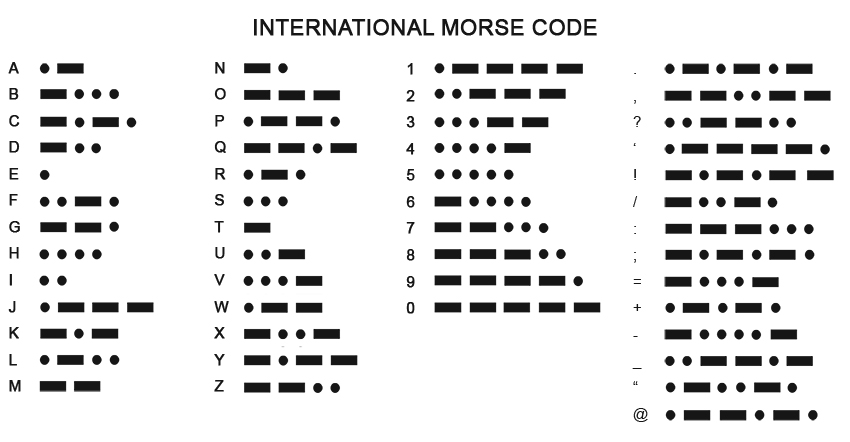
\includegraphics{Lossless_I/MorseCode.jpg}}
  \end{center}
\bit
\item Length of a dot is one unit.
\item Length of a dash is three units.
\item Space between parts of the same letter is one unit.
\item Space between letters is three units.
\item Space between words is seven units.
\eit
\end{frame}




\begin{frame}{Lossless Coding Scenario}
\begin{center}
\tikzstyle{encdec} = [rectangle, rounded corners, minimum width=2cm, minimum height=1cm,text centered, align=center, text width=2cm, draw=black]
\tikzstyle{iomsg} = [rectangle, rounded corners, minimum width=2cm, minimum height=1cm,text centered, text width=2.5cm, draw=black, fill=red!30]
\tikzstyle{arrow} = [thick,->,>=stealth]
\begin{tikzpicture}[node distance=2cm]
\node (inmsg) [iomsg] {Input Message\\ \textbf{s}};
\node (enc) [encdec, right of = inmsg, xshift=1.5cm ] {Encoder:\\ $\textbf{b}=\gamma(\textbf{s})$};
\node (dec) [encdec, right of = enc, xshift=2.5cm ] {Decoder:\\ $\textbf{s}=\gamma^{-1}(\textbf{b})$};
\node (outmsg) [iomsg, right of = dec, xshift=1.5cm ] {Output Message\\ \textbf{s}};
\draw [arrow] (enc) -- node[anchor=south] {bit-stream $\mathbf{b}$} (dec);
\draw [arrow] (enc) -- node[anchor=north] {$\mathbf{b}=00101$} (dec);
\draw [arrow] (inmsg) -- (enc);
\draw [arrow] (dec) -- (outmsg);
\end{tikzpicture}
\end{center}
\bit
\item \loud{Encoder:} Convert message $\mathbf{s}$ to bit-stream $\mathbf{b}$. Transmit $\mathbf{b}$.
\item \loud{Decoder:}  Parse $\mathbf{b}$ and convert back to message $\mathbf{s}$.  
\item[\iarrow] \ALERT{Decoder can exactly recover message from bitstream by inverting encoder operation.}
\eit
\smallskip
%\bit
%\item 
\loud{Bit rate reduction only possible if source messages $\mathbf{s}$ have statistical properties that can be exploited for compression. }
%\eit
\end{frame}





\begin{frame}{Lossless coding framework}
\loud{Messages:}
\begin{itemize}
%\item Reversible transmission of messages:
%\begin{itemize} 
%\item Encoder transmits message by converting it to a bit-sequence. 
%\item Decoder receives only bit-sequence, but can uniquely recover bit-sequence from message.  
%\end{itemize}
\item Assume that a \textbf{finite alphabet} $\mathcal{A}=\{a_1,\dots,a_N\}$ of \textbf{source symbols} $a_k$ is given. 
\item A \textbf{message} is a finite sequence $\textbf{s}=(a_{k_1},\dots,a_{k_l})$ of source symbols.
\item Write $\mathcal{A}^{<\infty}$ for the set of messages. 
\end{itemize}
\loud{Importance of lossless coding:}
\bit
\item Important in its own right. Lossless transmission might be desirable (Zip, PNG,...).
\item Even lossy compression systems (audio, image, video compression) contain lossless part:
\bit
\item Loss in information arises from quantization. All other parts are (more or less) lossless.
\item Before transmitting message, encoder can exactly compute quantization error and can adjust quantization stepsize
to required quality.  
\item Lossless transmission guarantees that error computed by encoder equals error in decoded message.  
\eit
\eit
\end{frame}

\section{Uniquely decodable codes}
\begin{frame}{Uniquely decodable codes}
\loud{Code}
\bit
\item Let $\mathcal{B}^{<\infty}$ denote the set of finite binary sequences. A \textbf{code} is a mapping 
\[
\gamma: \mathcal{A}\longrightarrow \mathcal{B}^{<\infty}. 
\]
\item The bit-sequences $\gamma(a_k)$ are called \textbf{codewords}.
\eit
\loud{Non-singular code}
\bit
\item A code is called \textbf{non-singular} if  $\gamma$ is injective, i.e. if 
$\gamma(a_i)\neq \gamma(a_j)$ for all $ a_i\neq a_j$. 
\eit 
\loud{Uniquely decodable code}
\bit
\item A code induces a mapping $\gamma^{<\infty}:\mathcal{A}^{<\infty}\to\mathcal{B}^{<\infty}$, 
\begin{align*}
\gamma^{<\infty}\left((a_{k_1},\dots,a_{k_l})\right):=\left[\gamma(a_{k_1}),\dots,\gamma(a_{k_l})\right],
\end{align*}
$[\:]$ the concatenation of sequences. 
\item A code is called \textbf{uniquely decodable} if $\gamma^{<\infty}$ is injective.
\item Uniquely decodable: Each bit-sequence arises by at most one message. 
\eit
\end{frame}

\section{Examples of codes}
\begin{frame}{Example: Variable-Length Coding for Scalars}
  \vspace{-1.5ex}
  \bit\TabPositions{9.2em,22.5em}
\item Symbol alphabet:
  $\set{A}=\{{\color{red}{\text{A}}},
  {\color{officegreen}{\text{B}}},
  {\color{saddlebrown}{\text{M}}},{\color{blue}{\text{N}}}\}$
\item<2->[]~\\[-1ex]
  {\relsize{-1}
  \begin{minipage}{0.32\linewidth}
    \begin{center}
      {\bf code~A}\\[.5ex]
      \begin{tabular}{|c|l|}
        \hline
    \color{black}letter & \color{black}codeword\\
    \hline\rule{0ex}{2.5ex}%
    \color{red}{A}         & ~~~\color{red}{00}\\
    \color{officegreen}{B} & ~~~\color{officegreen}{01}\\
    \color{saddlebrown}{M} & ~~~\color{saddlebrown}{10}\\
    \color{blue}{N}        & ~~~\color{blue}{11}\\
        \hline
    \end{tabular}
    \end{center}
  \end{minipage}
  \begin{minipage}{0.32\linewidth}
    \uncover<5->{\begin{center}
      {\bf code~B}\\[.5ex]
      \begin{tabular}{|c|l|}
        \hline
    \color{black}letter & \color{black}codeword\\
    \hline\rule{0ex}{2.5ex}%
    \color{red}{A}         & ~~~\color{red}{010}\\
    \color{officegreen}{B} & ~~~\color{officegreen}{100}\\
    \color{saddlebrown}{M} & ~~~\color{saddlebrown}{10}\\
    \color{blue}{N}        & ~~~\color{blue}{0}\\
        \hline
    \end{tabular}
    \end{center}}
    \end{minipage}
  \begin{minipage}{0.32\linewidth}
    \uncover<7->{\begin{center}
      {\bf code~C}\\[.5ex]
      \begin{tabular}{|c|l|}
        \hline
    \color{black}letter & \color{black}codeword\\
    \hline\rule{0ex}{2.5ex}%
    \color{red}{A}         & ~~~\color{red}{0}\\
    \color{officegreen}{B} & ~~~\color{officegreen}{110}\\
    \color{saddlebrown}{M} & ~~~\color{saddlebrown}{111}\\
    \color{blue}{N}        & ~~~\color{blue}{10}\\
        \hline
    \end{tabular}
    \end{center}}
  \end{minipage}\\[4ex]
  }
\item<3-> Example message: \tab$\ve{s}=\text{``{\color{officegreen}{B}\color{red}{A}\color{blue}{N}\color{red}{A}\color{blue}{N}\color{red}{A}\color{saddlebrown}{M}\color{red}{A}\color{blue}{N}}''}$
\item<4->[\iarrow] Bitstream (code A): \tab$\ve{b}=\text{``{\color{officegreen}{01}\color{red}{00}\color{blue}{11}\color{red}{00}\color{blue}{11}\color{red}{00}\color{saddlebrown}{10}\color{red}{00}\color{blue}{11}}''}$
  \tab(18 bits)
  \item<6->[\iarrow] Bitstream (code B): \tab$\ve{b}=\text{``{\color{officegreen}{100}\color{red}{010}\color{blue}{0}\color{red}{010}\color{blue}{0}\color{red}{010}\color{saddlebrown}{10}\color{red}{010}\color{blue}{0}}''}$
  \tab(20 bits)
  \item<8->[\iarrow] Bitstream (code C): \tab$\ve{b}=\text{``{\color{officegreen}{110}\color{red}{0}\color{blue}{10}\color{red}{0}\color{blue}{10}\color{red}{0}\color{saddlebrown}{111}\color{red}{0}\color{blue}{10}}''}$
    \tab(16 bits)
%  \item<9->[\ALERT{\iarrow}]\medskip\smallskip\ALERT{Goal: Minimize average codeword length}
%    \vspace{-1ex}$$
%    \usebeamercolor{alerted text}\color{fg}\bar{\ell}=\EV{\ell(S)}=\sum_kp_k\cdot\ell_k
%    $$
%\item Code A and code C: \tab uniquely decodable.
%\item Code B: \tab not uniquely decodable. 
  \eit\vspace{-10ex}
  \end{frame}





\begin{frame}{Example: Variable-Length Coding for Scalars}
  \vspace{-1.5ex}
  \bit\TabPositions{9.2em,22.5em}
\item Symbol alphabet:
  $\set{A}=\{{\color{red}{\text{A}}},
  {\color{officegreen}{\text{B}}},
  {\color{saddlebrown}{\text{M}}},{\color{blue}{\text{N}}}\}$
\item[]~\\[-1ex]
  {\relsize{-1}
  \begin{minipage}{0.32\linewidth}
    \begin{center}
      {\bf code~A}\\[.5ex]
      \begin{tabular}{|c|l|}
        \hline
    \color{black}letter & \color{black}codeword\\
    \hline\rule{0ex}{2.5ex}%
    \color{red}{A}         & ~~~\color{red}{00}\\
    \color{officegreen}{B} & ~~~\color{officegreen}{01}\\
    \color{saddlebrown}{M} & ~~~\color{saddlebrown}{10}\\
    \color{blue}{N}        & ~~~\color{blue}{11}\\
        \hline
    \end{tabular}
    \end{center}
  \end{minipage}
  \begin{minipage}{0.32\linewidth}
    {\begin{center}
      {\bf code~B}\\[.5ex]
      \begin{tabular}{|c|l|}
        \hline
    \color{black}letter & \color{black}codeword\\
    \hline\rule{0ex}{2.5ex}%
    \color{red}{A}         & ~~~\color{red}{010}\\
    \color{officegreen}{B} & ~~~\color{officegreen}{100}\\
    \color{saddlebrown}{M} & ~~~\color{saddlebrown}{10}\\
    \color{blue}{N}        & ~~~\color{blue}{0}\\
        \hline
    \end{tabular}
    \end{center}}
    \end{minipage}
  \begin{minipage}{0.32\linewidth}
    {\begin{center}
      {\bf code~C}\\[.5ex]
      \begin{tabular}{|c|l|}
        \hline
    \color{black}letter & \color{black}codeword\\
    \hline\rule{0ex}{2.5ex}%
    \color{red}{A}         & ~~~\color{red}{0}\\
    \color{officegreen}{B} & ~~~\color{officegreen}{110}\\
    \color{saddlebrown}{M} & ~~~\color{saddlebrown}{111}\\
    \color{blue}{N}        & ~~~\color{blue}{10}\\
        \hline
    \end{tabular}
    \end{center}}
  \end{minipage}\\[4ex]
  }
  \eit
  \vspace{-2ex}{\bf Decoding:}
  \bit\TabPositions{4.5em,18em}
\item<2-> Code A:\tab$\ve{b}=\text{``%
        \temporal< 3 >{01}{{\color{officegreen}01}}{{\color{gray!50}01}}%
        \temporal< 4 >{00}{{\color{red}00}}{{\color{gray!50}00}}%
        \temporal< 5 >{11}{{\color{blue}11}}{{\color{gray!50}11}}%
        \temporal< 6 >{00}{{\color{red}00}}{{\color{gray!50}00}}%
        \temporal< 7 >{11}{{\color{blue}11}}{{\color{gray!50}11}}%
        \temporal< 8 >{00}{{\color{red}00}}{{\color{gray!50}00}}%
        \temporal< 9 >{10}{{\color{saddlebrown}10}}{{\color{gray!50}10}}%
        \temporal<10 >{00}{{\color{red}00}}{{\color{gray!50}00}}%
        \temporal<11 >{11}{{\color{blue}11}}{{\color{gray!50}11}}%
  ``}$
  \tab\iarrow\quad$\ve{s}=\text{``%
        \temporal< 3>{}{{\color{officegreen}B}}{B}%
        \temporal< 4>{}{{\color{red}A}}{A}%
        \temporal< 5>{}{{\color{blue}N}}{N}%
        \temporal< 6>{}{{\color{red}A}}{A}%
        \temporal< 7>{}{{\color{blue}N}}{N}%
        \temporal< 8>{}{{\color{red}A}}{A}%
        \temporal< 9>{}{{\color{saddlebrown}M}}{M}%
        \temporal<10>{}{{\color{red}A}}{A}%
        \temporal<11>{}{{\color{blue}N}}{N}%
    \uncover<12->{``}}$

\item<13-> Code B:\tab$\ve{b}=\text{``%
  \temporal<14->{100}{{\color{magenta}100}}{100}%
  01000100010100100%
  ``}$
  \tab\iarrow\quad$\ve{s}=\text{``%
        \temporal<14->{}{{\color{officegreen}B} or {\color{saddlebrown}M}{\color{blue}N}}{?}%
        \uncover<14->{~...``}}$

\item<15-> Code C:\tab$\ve{b}=\text{``%
        \temporal<16 >{110}{{\color{officegreen}110}}{{\color{gray!50}110}}%
        \temporal<17 >{0}{{\color{red}0}}{{\color{gray!50}0}}%
        \temporal<18 >{10}{{\color{blue}10}}{{\color{gray!50}10}}%
        \temporal<19 >{0}{{\color{red}0}}{{\color{gray!50}0}}%
        \temporal<20 >{10}{{\color{blue}10}}{{\color{gray!50}10}}%
        \temporal<21 >{0}{{\color{red}0}}{{\color{gray!50}0}}%
        \temporal<22 >{111}{{\color{saddlebrown}111}}{{\color{gray!50}111}}%
        \temporal<23 >{0}{{\color{red}0}}{{\color{gray!50}0}}%
        \temporal<24 >{10}{{\color{blue}10}}{{\color{gray!50}10}}%
  ``}$
  \tab\iarrow\quad$\ve{s}=\text{``%
        \temporal<16>{}{{\color{officegreen}B}}{B}%
        \temporal<17>{}{{\color{red}A}}{A}%
        \temporal<18>{}{{\color{blue}N}}{N}%
        \temporal<19>{}{{\color{red}A}}{A}%
        \temporal<20>{}{{\color{blue}N}}{N}%
        \temporal<21>{}{{\color{red}A}}{A}%
        \temporal<22>{}{{\color{saddlebrown}M}}{M}%
        \temporal<23>{}{{\color{red}A}}{A}%
        \temporal<24>{}{{\color{blue}N}}{N}%
    \uncover<25->{``}}$
%  \item<26->[\ALERT{\iarrow}]\bigskip\ALERT{Necessary condition: Unique decodability:}\\[1ex]
%    \qquad\ALERT{Each bitstream uniquely represents a single message!}
  \eit%\vspace{-10ex}
  
    \vspace{-2ex}{\bf Unique decodability:}
    \bit\TabPositions{18em}
    \item Code A and Code C:\tab Uniquely decodable.
     \item Code B: \tab Not uniquely decodable. 
     \eit
  \end{frame}




\section{Probabilities of source symbols and average codeword length}
\begin{frame}{Probabilities of source symbols and average codeword length}
\loud{Known probability masses of source symbols}
\bit
\item Assume that symbols $a_k$ have known probabilities $p_k:=P(a_k)$.
\item The \loud{probability masses} $p_k$ satisfy
\begin{equation*}
\boxed{0 \leq p_k\leq 1 \:\forall k; \quad \sum_{k=1}^Np_k=1.} 
\end{equation*}
%\bit
%\item $0 \leq p_k\leq 1 \:\forall k$.
%\item $ \sum_{k=1}^Np_k=1$.
%\eit
\item Probabilstic framework enables mathematical theory of communication. Will be extended to stationary random processes 
and continuous probability distributions.
%\bit 
%\item Stationary random processes for lossless source coding. 
%\item Continous probability distributions for lossy source coding. 
%\eit
\eit 
\smallskip
\loud{Average codeword length:}
\bit
\item Let $\ell_k(\gamma)$ be the length of $\gamma(a_k)$. The average codeword length is defined as
\begin{align*}
\overline{\ell}(\gamma):=\sum_{k=1}^Np_k\cdot \ell_k(\gamma).
\end{align*} 
\item[\iarrow]\ALERT{Goal: Find uniquely decodable codes of minimal average codeword length.}
\eit
%\ALERT{Goal: Find uniquely decodable codes of minial average codeword length.}
\end{frame}



\section{Prefix codes}
\begin{frame}{Prefix codes}
\loud{Prefix codes}
\begin{itemize}
\item A \textbf{prefix code} is a non-singular code where no codeword is a prefix of a codeword different from it.
%\item Prefix code: If $a_1,\:a_2\in\mathcal{A}$, $a_1\neq a_2$, then $\cwd(a_1)\neq \cwd(a_2)$ and $\cwd(a_1)$ is not 
%a prefix of $\cwd(a_2)$.
\item Prefix codes are uniquely decodable.
\end{itemize}
\loud{Prefix codes as binary trees}
\begin{itemize} 
\item Prefix codes can always be represented by \textbf{binary trees}: 
\begin{itemize} 
\item Alphabet letters correspond to terminal nodes. 
\item Codewords are given by concatenation of labels on path from root to terminal nodes. 
\end{itemize}
\item Decoding of a bitstream: 
\bit
\item Start with root of binary tree. 
\item Read bit-by bit and follow code-tree from root until a terminal node is reached \\ $\rightarrow$ next codeword is decoded. 
\item Go back to root of binary tree.   
\eit
\end{itemize}
\end{frame}


\begin{frame}{Example of a prefix code}
A prefix code for the alphabet $\mathcal{A}=\{a,b,c,d,e\}$:
\begin{figure}
\begin{tikzpicture}%[edge from parent/.style={draw,-latex}]
[level distance=1.3cm,
  level 1/.style={sibling distance=4.0cm},
  level 2/.style={sibling distance=2.5cm}]
  \node [circle, draw]{}
    child {node [circle, draw]{}
      child {node [circle, draw,  fill=black, align=center, label=below:{a=(0,0)}]{} edge from parent node[ midway, left] {$0$}}
      child {node [circle, draw, fill=black,label=below:{b=(0,1)}]{} edge from parent node[ midway, right] {$1$}}
      edge from parent node[midway,left]{0}
    }
    child {node [circle, draw]{}
      child {node [circle, draw,fill=black,label=below:{c=(1,0)}]{}edge from parent node[midway,left]{0}}
      child {node [circle, draw]{}
      child{node[circle,draw, fill=black,label=below:{d=(1,1,0)}]{}edge from parent node[midway,left]{0}}      
      child{node[circle,draw, fill=black,label=below:{e=(1,1,1)}]{}edge from parent node[midway,right]{1}}
      edge from parent node[midway,right]{1}
      }
      edge from parent node[midway,right]{1}
    };
\end{tikzpicture}
%\caption{Example of a prefix code for the alphabet $\mathcal{A}=\{a,b,c,d,e\}$.}
\end{figure}
Example for bit-stream parsing: \textbf{bitstream}: 001100110111 $\mathbf{\rightarrow}$ \textbf{message}: adbce .
\end{frame}

\begin{frame}{Prefix code: Instantaneous decodability}
Prefix code not only uniquely decodable, but \loud{instantaneously decodable:}
\bit
\item Read bit by bit, can output symbol as soon as codeword is read. 
\item \loud{Advantage:} Decoder does not need to wait for whole bitstream to start decoding.
\eit 

\loud{Further advantage of instatenous decodability:} 
\bit
\item Mixture of different types of symbols (different alphabets) possible. 
\item In complex scenarios like video codec, order and presence of symbols is given by a \loud{syntax}. 
\item Example: Syntax elements can be prediction mode (motion vector or intra prediction mode) and prediction residual. 
\item Prefix code: Decoding with different codeword tables for different syntax elements possible:
\bit
\item Decode motion vector for given block with prefix code $A$.  
\item Decode prediction residual for block with prefix code $B$. 
\item Decode prediction mode of next block with prefix code $A$ ...
\eit
\eit

\end{frame}

\begin{frame}{Proper binary trees}
\loud{Proper binary trees:} 
\bit
\item A binary tree is called \loud{proper} if each node is either a leaf node or has two children.
\item A proper binary tree $\mathcal{T}_1$:
\begin{center}
\begin{forest}
for tree={%
    l sep=0.2cm,
    s sep=0.5cm
    }
[
 , circle, draw
     [
      , circle, draw
       [
        , circle, draw, fill
       ]
       [
        , circle, draw, fill
       ]
     ]
     [
      , circle, draw, fill
     ]
]
\end{forest}
\end{center}
\item A non-proper binary tree $\mathcal{T}_2$:

\begin{center}
\begin{forest}
for tree={%
    l sep=0.2cm,
    s sep=0.5cm
    }
[
 , circle, draw
     [
      , circle, draw
       [
        , circle, draw, fill
       ]
       [
        , circle, draw, fill
       ]
     ]
     [
      , circle, draw, color=red, fill
       [
         , circle, draw, fill
       ]
     ]
]
\end{forest}
\end{center}
\eit

\end{frame}

\begin{frame}{Proper binary trees and prefix codes without structural redundancy}
\loud{Decrease codeword-lengths by making tree proper:}
\bit
\item Let prefix code $\gamma$ be represented by binary tree $\mathcal{T}$.
\item Remove interior nodes of $\mathcal{T}$ that are a single child of 
other nodes.
\item Resulting tree $\mathcal{T}_{new}$ is proper. 
\item If $\gamma_{new}$ is prefix code corresponding to $\mathcal{T}_{new}$, then:
\bit
\item $\gamma_{new}$ can code the same number of symbols as $\gamma$.
\item For each symbol $a$, length of $\gamma_{new}(a)$ is smaller or equal than length of $\gamma(a)$. 
\eit
\item [\iarrow]\loud{Prefix code without structural redundancy: } Prefix code represented by proper binary tree.
\eit

\loud{Example}
\bit
\item Remove red interior 
node of $\mathcal{T}_2$ to obtain $\mathcal{T}_1$.
\item If $\gamma_2$ is code for $\mathcal{T}_2$, codewords of $\gamma_2$ are $\{00, 01, {\color{red}1}0 \}$.
\item If $\gamma_1$ is code for $\mathcal{T}_1$, codewords of $\gamma_1$ are $\{00, 01, 1 \}$.
\eit
\end{frame}


\begin{frame}{Path lengths for proper binary trees}
%\loud{Path lengths for proper binary trees}
\bit
\item Let $\mathcal{T}$ be a proper binary tree with leave node $\mathsf{n}$. 
\bit
\item Let $\mathsf{l}$ denote the length of the path from the root node of $\mathcal{T}$ to $\mathsf{n}$.
\item Create new binary tree $\mathcal{T}^{new}$ by appending two children $\mathsf{n}_1$ and $\mathsf{n}_2$ to
$\mathsf{n}$. 
\item Let $\mathsf{l}_1$ and $\mathsf{l}_2$ denote the lengths of paths to $\mathsf{n}_1$ and $\mathsf{n}_2$. Then:
\begin{align*}
2^{-\mathsf{l}}=2^{-\mathsf{l}_1}+2^{-\mathsf{l}_2}. 
\end{align*}
\eit 
\item [\iarrow] Induction on height of tree and number of nodes for given height: 
\begin{align*}
\sum_{k=1}^M2^{-\mathsf{l}_k}=1
\end{align*} 
for the lengths $\mathsf{l}_1,\dots,\mathsf{l}_M$ of paths to the nodes $n_1,\dots,n_M$ of any proper binary tree. 
\item [\iarrow] If $\mathcal{T}$ is any binary tree, prune to a proper binary tree as above. Path lengths decrease. Thus:  
\begin{align*}
\sum_{k=1}^M2^{-\ell_k}\leq 1
\end{align*}
holds for any binary tree.
\eit 
\end{frame}

\section{Kraft inequality and construction of prefix codes}
\begin{frame}{Kraft inequality for prefix codes} 
\begin{theorem}[Kraft inequality for prefix codes necessary and sufficient]
\bit 
\item \textbf{Kraft inequality:}
For a prefix code $\gamma$, one has 
\begin{align}\label{KraftPrefix}
\sum_{k=1}^N2^{-\ell_k}\leq 1
\end{align}
with equality if and only if $\gamma$ has no structural redundancy. 
\item \textbf{Conversely:} Given positive integers $\ell_1,\dots,\ell_N$ that satisfy \eqref{KraftPrefix}, there exists a prefix code such that the length of the $k$-th codeword is $\ell_k$. 
\eit 
\end{theorem} 
\loud{Proof of Kraft inequality:}
\bit
\item Follows immediately from above statements about path lengths of (proper) binary trees.
\eit
\loud{Proof of converse statement:}
\bit
\item Explicit construction of prefix code starting from perfect binary tree.
\eit
\end{frame}




%\begin{frame}{Proof of Kraft-MacMillan inequality}
%\loud{Preparation:}
%\begin{itemize}
%\item For $\ell, m\in\mathbb{N}$, let $K_{\ell}(m)$ denote the number of all messages of $m$ codewords that have combined length $\ell$. 
%\item There are only $2^\ell$ messages of length $\ell$, thus one has
%\begin{align}\label{upperK}
%K_\ell(m)\leq 2^\ell. 
%\end{align}
%\item Let $\ell_{\max}$ denote the maximal codeword length. 
%\item Trick: Take powers of $m$ of left hand side of \eqref{KraftMcMillan} and let $m\to\infty$. 
%\end{itemize}
%\end{frame}


\begin{frame}{Proof of converse statement}
\begin{itemize}
\item Assume $\ell_1\leq \ell_2\leq \dots\leq \ell_N=\ell_{max}$. 
\item Consider perfect binary tree $\mathcal{T}$ of height $\ell_{max}$: Unique binary tree of height $\ell_{max}$ with $2^{\ell_{max}}$ many leave nodes. 
\item Let $S_1$ denote the first $2^{\ell_{max}-\ell_1}$ leave nodes of $\mathcal{T}$, and inductively, for $j\leq N$ let $S_{j}$ denote the next $2^{\ell_{max}-\ell_j}$ leave nodes of $\mathcal{T}$.
\item By \eqref{KraftPrefix}, 
\begin{align*}
\sum_{k=1}^j2^{\ell_{max}-\ell_k}\leq 2^{\ell_{\max}}\cdot \sum_{k=1}^{N}2^{-\ell_k}\leq 2^{\ell_{max}}
\end{align*}
and thus each set $S_j$ is well defined.
\item Traverse each $S_k$ backward up to common root node $n_k$. If $S_k$ consist of one node, no backward traversion, $S_k=n_k$. 
\item Each root node $n_k$ is located at height $\ell_k$ within $\mathcal{T}$.
\item [\iarrow] The $n_k$ define code-words of length $\ell_k$.  
\item  Illustration of proof below.  

\end{itemize}
\qed
\end{frame}


\begin{frame}{Illustration of prefix code construction if Kraft inequality holds} 
\bit
\item Assume $\ell_1=1$, $\ell_2=2$, $\ell_3=3$, $\ell_4=3$. Thus:
\begin{align*}
2^{-\ell_1}+2^{-\ell_2}+2^{-\ell_3}+2^{-\ell_4}=1. 
\end{align*} 
\item Let $\mathcal{T}$ be perfect binary tree of height 3:
\begin{center}
\begin{forest}
[
 , circle, draw%, color=blue, fill
   [
   , circle, draw%, color=blue, fill
     [
       , circle, draw%, color=blue, fill
         [
           , circle, draw, color=blue, fill
         ]
         [
           , circle, draw, color=blue, fill
         ]
     ]
     [
       , circle, draw%, color=blue, fill
         [
           , circle, draw, color=blue, fill
         ]
         [
           , circle, draw, color=blue, fill
         ]
     ]
   ]
   [
   , circle, draw
     [
       , circle, draw%, color=red, fill
        [
         , circle, draw, color=red, fill
        ]
        [
         , circle, draw, color=red, fill
        ]
     ]
     [
      , circle, draw
        [
         , circle, draw, color =green, fill
        ]
        [
         , circle, draw, color = violet, fill
        ]
     ]
   ]
]
\end{forest}
.
\end{center}
\smallskip
\item Blue, red, green, and violet leave nodes comprise the sets $\mathcal{S}_1,\:\mathcal{S}_2, \:\mathcal{S}_3, \:\mathcal{S}_4$. 
\eit
\end{frame}




\begin{frame}{Illustration of prefix code construction if Kraft inequality holds} 
\bit
\item Move upwards from the node sets $\mathcal{S}_1,\:\mathcal{S}_2, \:\mathcal{S}_3, \:\mathcal{S}_4$ until a single root node is reached.
\item Here $\mathcal{S}_3$ and $\mathcal{S}_4$ are single nodes, thus no upward moving. 
\item Obtain 4 subtrees $\mathcal{T}_1,\:\mathcal{T}_2, \:\mathcal{T}_3, \:\mathcal{T}_4$. 
\begin{center}
\begin{forest}
[
 , circle, draw%, color=blue, fill
   [
   , circle, draw, color=blue, fill
     [
       , circle, draw, color=blue, fill
         [
           , circle, draw, color=blue, fill
         ]
         [
           , circle, draw, color=blue, fill
         ]
     ]
     [
       , circle, draw, color=blue, fill
         [
           , circle, draw, color=blue, fill
         ]
         [
           , circle, draw, color=blue, fill
         ]
     ]
   ]
   [
   , circle, draw
     [
       , circle, draw, color=red, fill
        [
         , circle, draw, color=red, fill
        ]
        [
         , circle, draw, color=red, fill
        ]
     ]
     [
      , circle, draw
        [
         , circle, draw, color =green, fill
        ]
        [
         , circle, draw, color = violet, fill
        ]
     ]
   ]
]
\end{forest}
.
\end{center}
\smallskip
\item Nodes of $\mathcal{T}_1,\:\mathcal{T}_2, \:\mathcal{T}_3, \:\mathcal{T}_4$ are drawn in blue, red, violet, green. 
\eit
\end{frame}









\begin{frame}{Illustration of prefix code construction if Kraft inequality holds} 
\bit
\item From $\mathcal{T}$, cut out all nodes of $\mathcal{T}_1,\:\mathcal{T}_2, \:\mathcal{T}_3, \:\mathcal{T}_4$ that are not parent nodes.
\item Resulting binary tree represents the prefix code with desired properties:
\begin{center}
\begin{forest}
for tree={%
    l sep=1.0cm,
    s sep=1.5cm
    }
[
 , circle, draw%, color=blue, fill
   [
   , circle, draw, color=blue, fill
   ]
   [
   , circle, draw
     [
       , circle, draw, color=red, fill
     ]
     [
      , circle, draw
        [
         , circle, draw, color =green, fill
        ]
        [
         , circle, draw, color = violet, fill
        ]
     ]
   ]
]
\end{forest}
.
\end{center}
\item Prefix code: {\color{blue}a}=0, {\color{red} b}=10, {\color{green}c}=110, {\color{violet}d}=111. 
\eit
\end{frame}



%\begin{frame}
%
%\begin{forest}
%[
% , circle, draw%, color=blue, fill
%   [
%   b
%     [
%       d
%         [
%           h
%         ]
%         [
%           i
%         ]
%     ]
%     [
%       e
%         [
%           j
%         ]
%         [
%           k
%         ]
%     ]
%   ]
%   [
%   , circle, draw
%     [
%       , circle, draw, color=red, fill
%        [
%         l
%        ]
%        [
%          m
%        ]
%     ]
%     [
%      g
%        [
%         n
%        ]
%        [
%         o
%        ]
%     ]
%   ]
%]
%\end{forest}
%\end{frame}





\section{Kraft-McMillan inequality}
\begin{frame}{Kraft-McMillan inequality}

Kraft inequality extends to arbitrary uniquely decodable codes:
\begin{theorem}[Kraft-McMillan inequality]
For any uniquely decodable code $\gamma$  one has
\begin{align}\label{KraftMcMillan}
\sum_{k=1}^N 2^{-\ell_k}\leq 1. 
\end{align}
\end{theorem}
\loud{Preparation for proof:}
\begin{itemize}
\item For $\ell, m\in\mathbb{N}$, let $K_{\ell}(m)$ denote the number of all bit sequences of length $\ell$ that arise from $m$ codewords under $\gamma^{<\infty}$. 
\item There are only $2^\ell$  bit sequences of length $\ell$, thus one has
\begin{align}\label{upperK}
K_\ell(m)\leq 2^\ell. 
\end{align}
\item Let $\ell_{\max}$ denote the maximal codeword length. 
\end{itemize}
\end{frame}

\begin{frame}{Proof of Kraft-MacMillan inequality}
\loud{Idea of proof:} Take powers of $m$ of left hand side of \eqref{KraftMcMillan} and let $m\to\infty$.
\begin{itemize}
\item %Trick: Take powers of $m$ of left hand side of \eqref{KraftMcMillan} and let $m\to\infty$.
 For every $m$ one has
\begin{align}\label{KraftPowerm}
\left(\sum_{k=1}^N 2^{-\ell_k}\right)^m & = \sum_{k_1=1}^N\cdots\sum_{k_m=1}^N2^{-\ell_{k_1}-\dots-\ell_{k_m}} \nonumber\\
&=\sum_{\ell=1}^{m\cdot \ell_{\max}}K_{\ell}(m)2^{-\ell}\nonumber\\
&\leq m\cdot \ell_{\max},
\end{align}
where the last inequality follows from \eqref{upperK}.
\item Since 
\begin{align*}
\lim_{m\to\infty}(m\cdot\ell_{\max})^{\frac{1}{m}}=1,
\end{align*} 
taking $m$-th rooth of left and right hand side of \eqref{KraftPowerm} proves \eqref{KraftMcMillan}. 
\end{itemize}
\qed 
\end{frame}







\begin{frame}{Consequences of Kraft-MacMillan and open question} 

%\loud{Possibility to check non-unique decodability:}  
%\bit
%\item Given code can not be uniquely decodable if \eqref{KraftMcMillan} does not hold for its codeword-lengths. 
%\eit

\loud{Suffices to consider prefix codes:} 
\bit 
\item For each uniquely decodable code, there exists a prefix code that has exactly the same codeword lengths.
\item Tree representing the corresponding prefix code can be constructed explicitly, see proof of converse statement of Kraft inequality. 
\eit

\ALERT{Open question:
Can one give lower and upper bounds for the optimal average codeword length achievable by any uniquely decodable code?}\\
\smallskip
\smallskip
\loud{Will be shown:}
\bit
\item Lower bound is given by the \loud{entropy} of the source-symbol distribution.
\item First upper bound: \loud{Shannon code}. Prefix code with average codeword length not greater than entropy plus 1.
\item Shannon code not always optimal, can have structural redundancies. Next lecture: \loud{Huffman codes}. 
\eit 


\end{frame}

\section{Kullback-Leibler divergence}
\begin{frame}{Kullback-Leibler divergence}
\begin{definition}[Kullback-Leibler divergence]
For two probability masses $p$ and $q$ on the symbol alphabet $\mathcal{A}$,  the number
\begin{align*}
D(p||q):=\sum_{k=1}^Np_k\log_2\left(\frac{p_k}{q_k}\right)
\end{align*}
is called the Kullback-Leibler divergence from $q$ to $p$. 
\end{definition}
Important property of Kullback-Leibler (KL) divergence: 
\begin{proposition}[Divergence Inequality]
One has $D(p||q)\geq 0$ with equality if and only if $p=q$.
\end{proposition}
\bit
\item Divergence inequality central for bounds of optimal average codeword length.
\item Sometimes also called Gibbs inequality. 
\eit
\end{frame}


\begin{frame}{Proof of Divergence Inequality. Preparation.}
\begin{lemma}[Elementary bound for natural logarithm]
One has $\ln(x)\leq x-1$ for all $x\in(0,\infty)$ and equality if and only if $x=1$.
\end{lemma} 
\loud{Proof of lemma: }
\begin{itemize}
\item Bernoulli inequality: 
\begin{align*}
(1+x)^{n}\geq 1+nx,\quad \forall x\in(-1,\infty), \quad \forall n\in\mathbb{N}. 
\end{align*}
and equality if and only if $n=1$ or $x=0$. Proof by induction on $n$.
\item Thus 
\begin{align}\label{IneqExp}
\exp(y)=lim_{n\to\infty}\left(1+\frac{y}{n}\right)^{n}\geq 1+y,\quad \forall y\in\mathbb{R} 
\end{align}
and equality if and only $y=0$. 
\item Setting  $y=\ln(x)$ in \eqref{IneqExp}, Lemma follows. $\qed$
\end{itemize} 
\end{frame}



\begin{frame}{Proof of Divergence Inequality}
One has: 
\begin{align*}
D(p||q)=&\sum_kp_k\log_2\left(\frac{p_k}{q_k}\right)\\
=&\frac{1}{\ln(2)}\sum_kp_k\ln\left(\frac{p_k}{q_k}\right)\\
=&-\frac{1}{\ln(2)}\sum_kp_k\ln\left(\frac{q_k}{p_k}\right)\\
\geq & \frac{1}{\ln(2)}\sum_kp_k\left(1-\frac{q_k}{p_k}\right) \tag {+}\label{Tag1}\\
=&\frac{1}{\ln(2)}\left(\sum_kp_k-\sum_kq_k\right)=0.
\end{align*}
Here, \eqref{Tag1} follows from previous lemma, equality if and only if $q_k=p_k$ for all $k$. $\qed$
\end{frame}

\section{Entropy and bounds for optimal average codeword length}
\begin{frame}{Entropy} 
\begin{definition}[Entropy of discrete pmf]
The entropy $H(p)$ of the discrete probability mass function $p$ is defined as
\begin{align*}
H(p):=\sum_{k=1}^N-p_k\cdot \log_2(p_k).
\end{align*}
\end{definition}
\bit 
\item Entropy is a measure of uncertainty for the distribution. 
\item If $N$ is the number of symbols in $\mathcal{A}$, then 
\[ 
H(p)\leq \log_2(N).
\] 
Equality if and only if $p$ is the uniform distribution, 
i.e. $p_k=1/N$ for all k.\\ $\rightarrow$ Maximal uncertainty for the uniform distribution. 
\item Proof: Exercise! Use Divergence Inequality.
\eit
\smallskip
\ALERT{
Entropy is central quantity to bound average code-length from below and above.
}  
\end{frame}



\begin{frame}{Entropy as lower bound for average codeword length}
\begin{theorem}[Entropy is lower bound for average codeword length]\label{TheoremEntr}
One has 
\begin{equation*}
\boxed{H(p) \leq \overline{\ell}(\gamma)} 
\end{equation*}
for any uniquely decodable code $\gamma$.
\end{theorem}
\loud{Main steps of proof}
\bit
\item Use \loud{Kraft-MacMillan inequality} and \loud{Divergence Inequality}. 
\item Let 
\begin{align*}
C:=\sum_{k=1}^N2^{-\ell_k}.
\end{align*}
\item Define a pmf $q$ by 
\begin{align}\label{DefqEntr}
q_k:=\frac{2^{-\ell_k}}{C}.
\end{align}
\eit
\end{frame}


\begin{frame}{Proof entropy lower bound for average codeword length}
One has
\begin{align*}
\overline{\ell}-H(p)=&\sum_kp_k\ell_k+\sum_kp_k\log_2(p_k)\\
=&-\sum_kp_k\log_2\left(2^{-\ell_k}\right)+\sum_kp_k\log_2(p_k)\\
%=&\sum_kp_k\log_2\left(\frac{p_k}{2^{-\ell_k}}\right)\nonumber\\
=&\sum_kp_k\log_2\left(\frac{p_k\cdot C}{2^{-\ell_k}\cdot C}\right)\\
=&\sum_kp_k\left(\log_2\left(\frac{p_k}{q_k}\right)-\log_2(C)\right)\\
=&D(p||q)-\sum_kp_k\log_2(C)\\
=&D(p||q)-\log_2(C).
\end{align*}
\loud{Divergence Inequality:} $D(p||q)\geq 0$. \\
\loud{Kraft-MacMillan Inequality:} $C\leq 1$, i.e. $-\log_2(C)\geq 0$ .  $\qed$
\end{frame}

\begin{frame}{Redundancy of a uniquely decodable code}
\loud{Redundancy: Measure of efficiency of a uniquely decodable code $\gamma$}.
\bit
\item Absolute redundancy: 
\begin{align*}
\rho(\gamma):=\overline{\ell}(\gamma)-H(p)\geq 0.
\end{align*}
\item Relative redundancy:
\begin{align*}
r(\gamma):=\frac{\overline{\ell}(\gamma)}{H(p)}\geq 1.
\end{align*}
\eit
\smallskip
\loud{Absolute redundancy zero if and only if each probability mass is negative integer power of two:}
\bit
\item If $p_k=2^{-i_k}$, $i_k\in\mathbb{N}$, by converse to Kraft-inequality, there exists a prefix-code $\gamma$ with lengths $\ell_k=i_k$. Obviously, 
$\overline{\ell}(\gamma)=H(p)$. 
\item Conversely, if $\rho(\gamma)=0$, then for pmf $q$ as in \eqref{DefqEntr}, proof of preceding theorem implies $D(p||q)=0$ and $C=1$. Thus 
$p_k=2^{-\ell_k}$. $\qed$
\eit
\end{frame}


\begin{frame}{Shannon Code}
\loud{Redundancy-free code not possible always possible, but:}
\bit 
\item For each $k\in\{1,\dots,N\}$ let 
\begin{align}\label{ShannonCode}
\ell_k:=\lceil-\log_2({p_k})\rceil.
\end{align}
\item One has  
\begin{align*}
\sum_k2^{-\ell_k}=&\sum_k2^{-\lceil-\log_2({p_k})\rceil}
\leq\sum_k2^{\log_2(p_k)}=1.
\end{align*}
\item Thus, by (converse) Kraft-inequality, there exists a prefix-code with codeword-lengths $\ell_k$ given by \eqref{ShannonCode}.
\item Such a code is called \loud{Shannon Code}.
\item Used to prove that entropy plus one is upper bound for optimal average codeword length. 
\eit
\end{frame}







\begin{frame}{Entropy plus one as upper bound for optimal average codeword length}
\begin{proposition}[Average codeword length not greater than entropy plus one possible]
There exists a uniquely decodable code whose average codeword length $\overline{\ell}(\gamma)$ satisfies
\begin{equation*}
\overline{\ell}(\gamma)\leq H(p)+1.
\end{equation*}
\end{proposition}
%Proof of proposition: 
%\bit
%\item 
\loud{Proof: Upper bound for average codeword length $\overline{\ell}$ of Shannon Code:}
%\item One has
\begin{align*}
\overline{\ell}=&\sum_kp_k\ell_k \\ =&\sum_kp_k\lceil-\log_2({p_k})\rceil\\ \leq &\sum_kp_k(-\log_2({p_k})+1) 
\\ =&H(p)+1.\qed 
\end{align*}
 %\eit
\end{frame} 


\end{document}
